\documentclass[11pt]{article}

\usepackage{makeidx}

\usepackage{latexsym}

\usepackage{color}

\usepackage{wrapfig}

\usepackage{here}

\usepackage{graphicx}

\usepackage[centertags]{amsmath}

\usepackage{amsfonts}

\usepackage{amssymb}

\usepackage{amsthm}

\usepackage{subfigure}

\usepackage{here}

\usepackage{ulsy}

\usepackage{hyperref}


\addtolength{\topmargin}{-2.5cm}

\addtolength{\textheight}{4cm}

\addtolength{\oddsidemargin}{-2cm} \addtolength{\textwidth}{3.5cm}

\addtolength{\evensidemargin}{-2cm}



\begin{document}

\renewcommand\floatpagefraction{.9}

\renewcommand\topfraction{.9}

\renewcommand\bottomfraction{.9}

\renewcommand\textfraction{.1}

\setcounter{totalnumber}{50} \setcounter{topnumber}{50}

\setcounter{bottomnumber}{50} \floatsep 20 pt \intextsep 5 pt

\abovecaptionskip 0 pt

\belowcaptionskip 0 pt



\newcommand{\beq}{\begin{equation}}

\newcommand{\eeq}{\end{equation}}

\newcommand{\ba}{\begin{array}}

\newcommand{\ea}{\end{array}}

\newcommand{\bea}{\begin{eqnarray}}

\newcommand{\eea}{\end{eqnarray}}

\newcommand{\bes}{\begin{eqnarray*}}

\newcommand{\ees}{\end{eqnarray*}}

\newcommand{\vs}{\vspace*{0.5cm}}

\newcommand{\svs}{\vspace*{0.25cm}}



\newcommand{\abs}[1]{\mid \! #1\! \mid}

\renewcommand{\b}[1]{\mbox{{\bf #1}}}

\renewcommand{\vec}[1]{\protect\overrightarrow{ #1}}

\newcommand{\mat}[1]{\mbox{\boldmath $#1$}}



\long\def\bform#1\eform{\begin{equation}

   \begin{minipage}{\eqbreite}\vskip .1cm

   \let\\ = \thcr

   \halign{$\displaystyle{##}$ \hfil

  && $\displaystyle{##}$\hfil\cr#1\cr}

   \vskip .3cm \end{minipage}

\end{equation}}

\def\thcr{\cr\noalign{\vskip.3cm}}

\newlength{\eqbreite}\setlength{\eqbreite}{\textwidth}

\addtolength{\eqbreite}{-1.5cm}



\long\def\bnn#1\enn{$$\begin{minipage}{\eqbreite}

\vskip .1cm \let\\ = \thcr \halign{$\displaystyle{##}$

\hfil && $\displaystyle{##}$\hfil \cr#1 \cr}

\vskip.3cm \end{minipage}$$}



\parindent 0 in

\parskip .25 cm



\input epsf



%%%%%%%%%%%%%%%%%%%%%%%%%%%%%%%%%%%%%%%%%%%%%%%%%%%%%%%%%%%

% Actual text starts below:

%%%%%%%%%%%%%%%%%%%%%%%%%%%%%%%%%%%%%%%%%%%%%%%%%%%%%%%%%%%



\thispagestyle{empty}

\svs

\begin{center}

\LARGE \textrm{\textbf{The Basic Stuff to Know - Mathematics Boot Camp: \\
 Introduction to Complex Systems Tools}}\\

\vspace*{1cm}  {\bf Viktor Jirsa} \\

\end{center} \vs



\normalsize
This intensive course is to provide students with the
prerequisites - some conceptual background and sufficient working
knowledge of mathematics - necessary to master the mathematically
based graduate courses at the Center for Complex Systems \& Brain
Sciences. By no means it is intended to compete with the
traditional introductory courses in mathematics taught at
universities. Rather it should be viewed as a synopsis of the
mathematical tools most probably encountered in scientific
applications. The present script is meant to serve as a companion
during the boot camp and as a quick reference and look-up source
after the boot camp.
\vs \svs



\begin{figure}[!h]

    \centerline{\epsfxsize=10cm  \epsfbox{FRONT_COVER.ps}}

\end{figure} \vs \svs



\begin{center} \Large

\textrm{Boca Raton Florida, August 2002 \\
     Center for Complex Systems and Brain Sciences \\
     Florida Atlantic University}
\end{center}  \normalsize



\newpage

\vspace{5cm}
\begin{center} \Large
  \textrm{{\bf LICENSE}\\
    \vs
    Copyright (c) 2018 Viktor K. Jirsa}
\end{center} \normalsize \vs \svs



This work is licensed under the Creative Commons Attribution-NonCommercial-ShareAlike 4.0 International License. 
To view a copy of this license, visit \href{http://creativecommons.org/licenses/by-nc-sa/4.0/}{this page} or send a letter 
to Creative Commons, PO Box 1866, Mountain View, CA 94042, USA.

\vspace{3cm}

\begin{figure}

    \centerline{\epsfxsize=11cm \includegraphics{CC-license.eps}}

\end{figure} \vs \svs



\newpage

\tableofcontents

\listoffigures



\newpage

\pagestyle{plain}



%\setcounter{page}{1}

\section{Function Theory}
\subsection{Foundations}

{\bf Definition:} A {\em function} $f$ is a rule which unambiguously
assigns $y \in B$ to each $x \in A$.

"$x \in A$" means that "$x$ is an element of $A$". \vs

\begin{figure}[!h]
    \centerline{\epsfxsize=11cm  \epsfbox{matlab/fig1.eps}} \vs
    \caption{Illustration of a function} \label{fig1}
\end{figure} \vs

{\bf Notation:}
\bnn \begin{array}{ccc}
    f: & A \rightarrow B & \\ \svs
    f: & A \rightarrow B & \;\; x\in A, \; y\in B \\ \svs
    & y = f(x) & \;\; x\in A, \; y\in B \\ \svs
    & y = y(x) & \;\; x\in A, \; y\in B
\end{array} \enn \vs

{\bf Examples:}

\vs \begin{figure}[!h]
   \centerline{\epsfxsize=11cm \epsfbox{matlab/fig2.eps}} \vs
   \caption{Assigning an element $\{21\} \in B$ to $\{1\} \in A$} \label{fig2}
\end{figure} \vs

\newpage

Most commonly, functions are defined by equations: $\qquad y = f(x) = 2x + 1 \qquad\quad y=f(x)=x^2$  \svs

{Graphical representation:} \svs
\begin{figure}[!h]
    \centering
    \subfigure[Function $y = 2x + 1$]{\epsfxsize=7cm \epsfbox{matlab/fig3a.eps}}
    \hspace*{0.5cm}
    \subfigure[Function $y = x^2$]{\epsfxsize=7cm \epsfbox{matlab/fig3b.eps}} \svs
    \caption{A linear and a quadratic function} \label{fig3}
\end{figure} \vs

\subsection{Inverse Functions}

$f^{-1}$ denotes the inverse of the function $f$. \vs

\begin{figure}[!h]
   \centerline{\epsfxsize=11cm  \epsfbox{matlab/fig4.eps}} \svs
    \caption{Inverse function} \label{fig4}
\end{figure} \vs

{\bf Notation:}
\bnn f^{-1}: \; B \rightarrow A \enn \svs
\bnn x = f^{-1}\,(y) \qquad \mbox{where} \qquad y = f(x) \enn \svs

Graphically the inverse can be constructed as the mirror image of the function at the
first bisector. This method always works, but caution is asked for, because the inverse 
may not be unique and require more detailed discussion.

{\bf Example:}
\bnn y = f(x) = 2x + 1  \qquad  x = f^{-1}\,(y) = \frac{1}{2} \, (y-1) \enn

{\bf Note:} There is not always an inverse function!  \vs

\begin{figure}[!h]
   \centerline{\epsfxsize=11cm \epsfbox{matlab/fig5.eps}} \svs
    \caption{The inverse $f^{-1}$ is not unique, thus not a function.} \label{fig5}
\end{figure} \vs


{\bf Example:}
\bnn y = f(x) = x^2 \enn
\bnn x = \sqrt{y} \qquad \mbox{or} \qquad x = -\sqrt{y} \enn  \vs

\begin{figure}[!h]
    \centering
    \subfigure[$\; f(x)=2\,x+1 \; \rightarrow \; f^{-1}(x)=\frac{1}{2}(x-1)$]{\epsfxsize=7cm \epsfysize=7cm
        \epsfbox{matlab/fig6a.eps}}
    \hspace*{0.5cm}
    \subfigure[$\; f(x)=x^2 \; \rightarrow \; f^{-1}(x)=\pm\sqrt{x}$]{\epsfxsize=7cm \epsfysize=7cm
         \epsfbox{matlab/fig6b.eps}} \svs
    \caption{Graphical construction of the inverse function} \label{fig6}
\end{figure}

\newpage
\subsection{Implicit Functions}
A function is not given explicitly as in $y = f(x)$, but
implicitly by $F(x,y) = 0$.

{\bf Example:} Unit circle: $\quad F(x,y)=x^2+y^2-1=0$. \svs

\begin{figure}[!h]
    \centerline{\epsfxsize=7cm \epsfysize=7cm \epsfbox{matlab/fig7.eps}} \svs
    \caption{Unit circle} \label{fig7}
\end{figure} \svs

The implicit representation of the unit circle also needs additional conditions to become
unique and thus a function: a local neighborhood has to be defined, e.g. $y=\sqrt{1-x^2}$
for \mbox{$x\in (-1;1)$},  \mbox{$y >0$} and $y=-\sqrt{1-x^2}$ for $x\in (-1;1), \, y<0$.

\subsection{Polynomials}
Polynomials are defined as a class of functions of the form
\bnn y = a_0 + a_1 \, x + a_2 \, x^2 + \dots + a_N \, x^N = \sum_{n=0}^N a_n \, x^n \enn
where the function $y$ is said to be a polynomial of order $N$.  \svs

{\bf Example:}
\bnn y = \underbrace{2}_{a_2} x^2 + \underbrace{8}_{a_1} x + \underbrace{4}_{a_0} \enn

{\bf Goal:} To achieve a qualitative understanding of a given function without computing each value.

{\bf Approach:}
\bnn y = \sum_{n=0}^N a_n \, x^n  \qquad \mbox{where we assume} \;\; a_N>0 \enn

\begin{description}
\item[{\bf Step 1:}] If $N$ is even, then $x \rightarrow \pm\infty : y \rightarrow \pm \infty \, ; \quad$
if $N$ is odd, then $x \rightarrow \pm \infty : y \rightarrow \mp \infty$. Note: If $a_N<0$,
the behavior is the opposite.
\item[{\bf Step 2:}] A polynomial of order $N$ has $N$ roots which are the solutions of $f(x)=0$.

Set $y=0: f(x) = x^N + a_{N-1}\, x^{N-1} + \dots + a_1 \,x + a_0 = 0 $
\bnn \begin{array}{ccl} \svs
y = 17x + 4 \quad & y=0: x=-\frac{4}{17} & \quad \rightarrow  \quad \mbox{1 root} \\
y = 2x^2 + 8x + 4 \quad & y=0: x=\frac{1}{4}(-8 \pm \sqrt{8^2-4\cdot2\cdot4})=\frac{1}{4}(-8 \pm
\sqrt{32)}=-2 \pm \sqrt{2} & \quad \rightarrow \quad  \mbox{2 roots}
\end{array} \enn
\begin{center}
    $\Rightarrow$ the roots are the locations where $f(x)$ crosses the $x$-axis.
\end{center}
\end{description}

{\bf Examples:} Construct graph of $y=f(x)$ \vs
\begin{figure}[!h]
\centering \subfigure[Step 1: $y=x^2+3x+2$] {\epsfxsize=7cm \epsfbox{matlab/fig8a.eps}}
\hspace*{0.5cm}
\subfigure[Step 2:  $y=x^2+3x+2=0$] {\epsfxsize=7cm \epsfbox{matlab/fig8b.eps}} \svs 
\caption{Graphical construction (the roots are $x=-1$ and $x=-2$)} \label{fig8}
\end{figure}

\vs\vs\begin{figure}[!h]
\centering \subfigure[Step 1: $y=x^3+2x^2-3x$] {\epsfxsize=7cm \epsfbox{matlab/fig9a.eps}}
\hspace*{0.5cm}%
\subfigure[Step 2: $y=x^3+2x^2-3x=0$] {\epsfxsize=7cm \epsfbox{matlab/fig9b.eps}} \svs 
\caption{Graphical construction (the roots are $x=-3, x=0$ and $x=1$)} \label{fig9}
\end{figure}

\begin{figure}[!h]
\centering \subfigure[Step 1: $y=x^4+2x^3-3x^2$] {\epsfxsize=7cm \epsfbox{matlab/fig10a.eps}}
\hspace*{0.5cm}%
\subfigure[Step 2: $y=x^4+2x^3-3x^2=0$] {\epsfxsize=7cm \epsfbox{matlab/fig10b.eps}} \svs 
\caption{Graphical construction (the roots are $x=-3, x=0$ and $x=1$)} \label{fig9}
\end{figure} 

\newpage

{\bf Horizontal translation} is a horizontal shift of a function by $x_0$
\bnn y=f(x) \; \rightarrow \; y =f(x-x_0) \enn

{\bf Example:} $\qquad y = x^2$  \; shift by $\; x_0=2$: \; $ y = (x-2)^2 = x^2 - 4x +4$  \vs

\vs {\bf Vertical translation} is a vertical shift of a function by $y_0$
\bnn y=f(x) \; \rightarrow \; y =f(x)+y_0 \enn

{\bf Example:} $\qquad y=x^2$ \; shift by $\; y_0=2$: \;  $ y=x^2+2 $ \vs

\vs\begin{figure}[!h]
\centering \subfigure[Horizontal shift by $x_0=2: y=(x-2)^2$]{\epsfxsize=7cm \epsfbox{matlab/fig11a.eps}} 
\hspace*{0.5cm}
\subfigure[Vertical shift by $y_0=2: y = x^2+2$] {\epsfxsize=7cm \epsfbox{matlab/fig11b.eps}} \svs 
\caption{Vertical and horizontal shift of $y=x^2$} \label{fig11}
\end{figure}

\subsection{Trigonometric Functions}
Trigonometric functions are a class of periodic functions such as
\bnn y = f(x) = A \sin(kx + \phi) \quad \mbox{and} \quad
     y = f(x) = A \cos(kx + \phi) \enn

The constant parameters are the amplitude
$A$, the frequency $k$ and the phase (angle) $\phi$. The period is
defined as $\lambda=2\pi/k$ and the trigonometric functions fulfill
the relation $f(x+\lambda)=f(x)$.
\small  \vspace*{-5mm} \begin{center} \begin{tabular}{|c|c|c|c|c|c|c|c|c|} \hline
\multicolumn{9}{|c|} {Special values of trigonometric functions (midnight stuff)\rule{0pt}{4mm}} \\
\hline \hline
$x$ & $\;0\;$ & $\pi/6=30^{\circ}$ & $\pi/4=45^{\circ}$ & $\pi/3=60^{\circ}$ & $\;\pi/2=90^{\circ}\;$ & $\;\pi=180^{\circ}\;$
 & $\;3\pi/2=270^{\circ}\;$ & $\;2\pi=360^{\circ}\; $  \rule{0pt}{4mm} \\
\hline
$\;\sin x\;$ & $0$ & $1/2$ & $\sqrt{2}/2$ & $\sqrt{3}/2$ & $1$ & $0$ & $-1$ & $0$  \rule{0pt}{4mm} \\
\hline
$\cos  x$    & $1$ & $\sqrt{3}/2$ & $\sqrt{2}/2$ & $1/2$ & $0$ & $-1$ & $0$ & $1$ \rule{0pt}{4mm} \\
\hline
\end{tabular} \end{center} \normalsize

Horizontal translation (shift) by means of $\phi$:
\bnn
\sin(x+\frac{\pi}{2})=\cos{x} \qquad \cos(x+\frac{\pi}{2})=-\sin{x} \qquad
\sin(x-\frac{\pi}{2})=-\cos{x} \qquad \cos(x-\frac{\pi}{2})=\sin{x}
\enn

Useful relations between $\cos{x}$ and $\sin{x}$:
\bnn \cos^2{x}+\sin^2{x}=1 \enn
\bnn \sin(x\pm y)=\sin{x}\cos{y} \pm \cos{x}\sin{y} \qquad
\cos(x\pm y) = \cos{x}\cos{y} \mp \sin{x}\sin{y} \enn
\bnn \sin{2x} = 2\sin{x}\cos{x} \qquad
\cos{2x} = \cos^2{x} - \sin^2{x} \enn

Other trigonometric functions:
\bnn \tan{x} = \frac{\sin{x}}{\cos{x}} \qquad\qquad \cot{x} = \frac{\cos{x}}{\sin{x}} \enn

\begin{figure}[!h]
\centering 
\subfigure[The functions  $y\!=\!\sin{x}$ and \mbox{$y\!=\!\cos{x}$}] {\epsfxsize=7cm \epsfbox{matlab/fig12a.eps}}
\hspace*{0.5cm}
\subfigure[The functions $y\!=\!\tan{x}$ and $y\!=\!\cot{x}$. Note that these are $\pi$-periodic]
           {\epsfxsize=7cm \epsfbox{matlab/fig12b.eps}} \svs
\caption{The most common trigonometric functions} \label{fig12}
\end{figure}


\subsection{Exponential Functions}

Exponential functions are functions most commonly used in the form
\bnn y = A e^{kx} = A \exp{k x} \enn
with the constant parameters: $A$ amplitude, $k$ growth rate if $k>0$ and the damping or fall 
off, if $k<0$, and $e$ Euler number: 2.714....

Note that $e^0=1\;$ and $\;e^{-x}=\frac{1}{e^x}$. \svs

\begin{figure}[!h]
    \centerline{\epsfxsize=10cm \epsfbox{matlab/fig13.eps}}
    \caption{Exponential functions} \label{fig13}
\end{figure} \vs


\subsection{Hyperbolic Functions}

Hyperbolic functions are of the form
\bnn y = f(x) = \cosh{x} = \frac{1}{2}(e^x + e^{-x}) \qquad\mbox{hyperbolic cosine} \enn
and
\bnn y = f(x) = \sinh{x} = \frac{1}{2}(e^x - e^{-x}) \qquad\mbox{hyperbolic sine} \enn

They have similar properties as the trigonometric functions such as a representation by
exponentials (as we shall see later), and their derivatives convert into each other. 
But the hyperbolic functions are {\em not} periodic. \vs

Other hyperbolic functions:
\bnn
y=\tanh{x}=\frac{\sinh{x}}{\cosh{x}}=\frac{e^{x}-e^{-x}}{e^{x}+e^{-x}} \qquad
y=\coth{x}=\frac{\cosh{x}}{\sinh{x}}=\frac{e^{x}+e^{-x}}{e^{x}-e^{-x}}
\enn

\begin{figure}[!h]
    \centering
    \subfigure[$y=\sinh{x}\;$ and $\;y=x+\frac{1}{3!}\,x^3$]{\epsfxsize=7cm \epsfbox{matlab/fig14b.eps}}
    \hspace*{0.5cm}
    \subfigure[$y=\cosh{x}\;$ and $\;y=1+\frac{1}{2!}\,x^2$]{\epsfxsize=7cm \epsfbox{matlab/fig14a.eps}} \svs
    \caption{Hyperbolic functions} \label{fig14}
\end{figure} \vs



\subsection{Basic Inverse Functions}
\subsubsection{Logarithms}
The logarithms are the inverse of the exponential functions:
\bnn y=a^x \quad \leftrightarrow \quad x = \log_a y  \qquad\mbox{where} \quad 0<y<\infty \enn

{\bf Special cases:}
\begin{eqnarray*}
\begin{array}{lcccccc}
a=e: \qquad & y & = & \log_e x & = & \ln x & \qquad\mbox{natural logarithm}\\
a=10: \qquad & y & = & \log_{10} x & = & \mbox{lg} x & \qquad\mbox{decimal logarithm}\\
a=2: \qquad  & y & = & \log_2 x & = & \mbox{ld} x & \qquad\mbox{dual logarithm}
\end{array}
\end{eqnarray*}

\begin{figure}[!h]
    \centerline{\epsfxsize=10cm  \epsfbox{matlab/fig15.eps}} \svs
   \caption{The logarithmic functions $y=\ln(x)$, $y=\mbox{lg}(x)$, $y=\mbox{ld}(x)$, and $y=-\ln(x)$.} \label{fig15}
\end{figure} \vs

{\bf Remark:} The most commonly used logarithm is $\ln x$, but there are certain applications for other 
logarithms as well. For instance, the decimal logarithm can be used to find the number of digits in 
a decimal number 
($\mbox{lg} 4821=3.683 \rightarrow$  taking the whole number in front of the decimal point and 
adding 1 gives the number of digits, 4). Similarly, the dual logarithm can be used to find the number
of bits or binary digits that are necessary to represent a number $n$ in binary format, i.e. as 
zeros and ones.  

{\bf Rules and tricks for dealing with logarithms:}
\bnn \ln x^n = n \ln x \enn
\bnn \ln x_1 \, x_2 = \ln x_1 + \ln x_2  \qquad  \ln \frac{x_1}{x_2} = \ln x_1 - \ln x_2  \enn
\bnn \log_a x = \frac{\ln x}{\ln a} \enn

{\bf Note:} Every logarithm can be expressed in terms of the natural logarithm, and every exponential 
function can be written in terms of the basis $e$
\bnn    a^x = e^{x\,\ln a} \quad \mbox{with} \quad a>0 \qquad \mbox{\bf Very useful relation!} \enn 

\subsubsection{Other inverse functions}
\vspace*{-0.9cm} \begin{eqnarray*} \begin{array}{llll}
y=\sin x & \rightarrow & x = \arcsin y & \mbox{arc sine} \\
y=\cos x & \rightarrow & x = \arccos y & \mbox{arc cosine} \\
y=\tan x & \rightarrow & x = \arctan y & \mbox{arc tangent} \\
y=\cot x & \rightarrow & x = \mbox{arccot } y & \mbox{arc cotangent} \\
y=\sinh x & \rightarrow & x = \mbox{arcsinh } y & \\
& & x=\ln(y+\sqrt{y^2+1})
& \mbox{area sine hyperbolic} \\
y=\cosh x & \rightarrow & x = \mbox{arccosh } y & \\
& & x = \ln(y+\sqrt{y^2-1})
& \mbox{area cosine hyperbolic}
\end{array} \end{eqnarray*} \svs

\begin{figure}[!h]
    \centering
    \subfigure[Arc sine, and arc cosine]{\epsfxsize=7cm \epsfbox{matlab/fig15_1a.eps}}
    \hspace*{0.5cm}
    \subfigure[Arc tangent, and arc cotangent]{\epsfxsize=7cm \epsfbox{matlab/fig15_1b.eps}} \svs
    \caption{The inverse of the trigonometric functions}
\end{figure}

\subsection{Elementary Combinations of Functions}
\subsubsection{Superposition}
Two functions are superimposed on each other by adding their values for the same $x$.
\bnn y = f_1(x) + f_2(x) \enn
\vspace*{-.5cm} \begin{figure}[!h]
    \centering
    \subfigure[Superposition of $f_1(x)\!=\!-x \mbox{ and } f_2(x)\!=\!1$]{\epsfxsize=7cm \epsfbox{matlab/fig16a.eps}}
    \hspace{0.5cm}
    \subfigure[Superposition of $f_1(x)\!=\!-2x \mbox{ and } f_2(x)\!=\!x^3$]{\epsfxsize=7cm \epsfbox{matlab/fig16b.eps}} \svs
    \caption{Superposition of lines and functions} \label{fig17}
\end{figure}

\subsubsection{Modulation}
A function is modulated by another function by multiplying their values for the same $x$. 
\bnn y = f_1(x) \, f_2(x) \enn

\vs\begin{figure}[!h]
    \centering
    \subfigure[$e^{-x}$ is the envelope function of $\cos 10x$] {\epsfxsize=7cm \epsfbox{matlab/fig17a.eps}}
    \hspace{0.5cm}
    \subfigure[$\cos 10x$ is modulated with $\sin x$]{\epsfxsize=7cm \epsfbox{matlab/fig17b.eps}}  \svs
    \caption{Modulation of functions} \label{fig19}
\end{figure}
  \newpage


% \setcounter{page}{12}

\section{Differential and Integral Calculus}\label{diff}
First derivatives of simple functions were studied by Galileo
Galilei (1564-1642) and Johannes Kepler (1571-1630). A systematic
theory of differential calculus was developed by Isaac Newton
(1643-1727) and Gottfried Wilhelm Leibniz (1646-1710).

\subsection{Difference Quotient}
The difference quotient becomes the differential in the limit
$h\rightarrow 0$ and describes the slope of a function $y=f(x)$
at a given point $x$.
\bnn y'(x)=\frac{dy}{dx}=\underset{h\rightarrow0}{\lim} \frac{y(x+h) - y(x)}{h} \enn

\begin{figure}[!h]
    \centerline{\epsfxsize=10cm \epsfysize=9cm \epsfbox{matlab/fig18.eps}} \svs
    \caption{The slope of a curve is found from its derivative.} \label{fig20}
\end{figure} \vs

\begin{figure}[!h]
    \centerline{\epsfxsize=10cm \epsfbox{matlab/fig19.eps}} \svs
    \caption{Slope as h$\rightarrow 0$.} \label{fig21}
\end{figure} \svs

{\bf Notation:} The limit value of the difference quotient is called the
derivative of a function $f(x)$. Derivatives are denoted by
\bnn y'(x)\;,\;\frac{dy}{dx}\;,\;\frac{df}{dx}\;,\;\frac{d}{dx}f(x) \qquad
\mbox{or sometimes in physics:} \;\; \dot{y}(t) \enn

{\bf Note:} Here we consider first-order derivatives only.

\vs
{\bf Example:}  $\qquad y = f(x) =x^2$
\bnn
y'\,=\,\frac{dy}{dx}=\underset{h\rightarrow 0}{\lim} \frac{(x+h)^2-x^2}{h}
\,=\,\underset{h\rightarrow 0}{\lim} \frac{x^2 +2hx +h^2 -x^2}{h}
\,=\,\underset{h\rightarrow 0}{\lim} \frac{2hx+h^2}{h} = 2x
\enn \vs

\subsection{Derivatives of Elementary Functions}

\subsubsection{Polynomials}
\vspace*{-2mm}\bnn y=x^2 \quad \rightarrow \quad \frac{dy}{dx}=2x
\qquad \qquad \qquad \mbox{more general:} \quad
y=x^n \quad \rightarrow \quad \frac{dy}{dx}=nx^{n-1} \enn

\subsubsection{Trigonometric functions}
\vspace*{-2mm}\bnn
y=\sin x \quad \rightarrow \quad \frac{dy}{dx}=\cos x \qquad \qquad \qquad
y=\cos x \quad \rightarrow \qquad \frac{dy}{dx}=-\sin x
\enn

\subsubsection{Exponential functions}
\vspace*{-2mm}\bnn y=e^x \quad \rightarrow \quad \frac{dy}{dx}=e^x \enn

\subsubsection{Hyperbolic functions}
\vspace*{-2mm}\bnn
y=\sinh x \quad \rightarrow \quad \frac{dy}{dx}=\cosh x \qquad \qquad \qquad
y=\cosh x \quad \rightarrow \quad \frac{dy}{dx}=\sinh x
\enn

\subsubsection{Logarithms}
\vspace*{-2mm}\bnn y=\ln x \quad \rightarrow \quad \frac{dy}{dx}=\frac{1}{x} \enn

\subsection{The Basic Rules for Calculating Derivatives}
If the derivatives of two functions $u(x)$ and $v(x)$ exist on an interval
$a<x<b$, then the derivatives of their combinations exist as well, i.e.
\bnn
u+v, \quad \alpha \, u \;\; \mbox{with} \;\; \alpha \in \mathbb{R}, \quad
u\,v, \quad \frac{u}{v} \;\; \mbox{if} \;\; v(x)\not=0 \;\; \mbox{for} \;\; a<x<b
\enn
{\bf Rules:}
\bnn \begin{array}{cc} \svs
\qquad (u + v)'=\frac{d}{dx}\{u+v\}=u' + v' & \qquad\qquad \mbox{\bf derivatives are additive} \qquad\qquad \\ \svs
\qquad (\alpha \, u)'=\frac{d}{dx}\{\alpha \, u\}=\alpha \, u' & 
\qquad\qquad \mbox{\bf multiplication with a scalar} \qquad\qquad \\ \svs
\qquad (u\,v)'=\frac{d}{dx}\{u\,v\}= u'\,v+u\,v'  & \qquad\qquad \mbox{\bf product rule} \qquad\qquad \\ \svs
\qquad (\frac{u}{v})'=\frac{d}{dx}\{\frac{u}{v}\}=\frac{u'\,v - u\,v'}{v^2} & \qquad\qquad \mbox{\bf quotient rule} \qquad\qquad
\end{array} \enn

{\bf Examples:}
\bnn \frac{d}{dx}\{x^{17}+\cos x\} = 17x^{16}-\sin x \enn
\bnn \frac{d}{dx}\{35 \cosh x\}=35 \frac{d}{dx}\,\cosh x=35 \sinh x \enn
\bnn \frac{d}{dx}\{\cos x e^x\} = - \sin x e^x +\cos x e^x = e^x (\cos x - \sin x) \enn
\bnn \frac{d}{dx}\{\frac{\cos x}{e^x}\} = \frac{-\sin x \, e^x - \cos x \, e^x}{e^{2x}}
    =\frac{-e^x \, (\sin x +\cos x)}{e^{2x}}= -\frac{\sin x + \cos x}{e^x} \enn \svs


\subsection{The Chain Rule}
If $u(x)$ and $v(x)$ have derivatives and the image of $v(x)$ is part of the source set of $u(x)$, 
then $u(v(x))$ has a derivative. 

To understand what this complicated sentence means, consider 
$\ln(\cos x)$. Here $u(x)=\ln x$ and $v(x)=\cos x$. The source set of $\cos x$ are all real numbers
$[-\infty, \infty]$, the image set of the cosine are the numbers in the interval [-1, 1], and the source 
set of the logarithm are all positive real numbers $]0, \infty]$. Therefore the image set of the cosine 
and the source set of the logarithm overlap in the interval $]0, 1]$. The source set of $\cos x$ that corresponds
to the image set $]0, 1]$ is given by all numbers where $\cos x$ is positive, i.e. $]-\frac{\pi}{2}, -\frac{\pi}{2}[$,
$]\frac{3\,\pi}{2}, -\frac{5\,\pi}{2}[$, etc., and the function $\ln(\cos x)$ exists and has a derivative for 
these values of $x$.
\bnn [u(v(x))]'=\frac{d}{dx}\{u(v(x))\}= \frac{d\,u(v)}{dv}\;\frac{d\,v(x)}{dx} \qquad\qquad \mbox{\bf chain rule} \enn

{\bf Examples:}
\bnn f(x)=\cos(\alpha x) \quad \rightarrow \quad u(v)=\cos v \quad \mbox{and} \quad v(x)=\alpha x \enn
\bnn \frac{d}{dx}\,\cos \alpha x=\frac{d\,\cos \alpha x}{d\,\alpha x}\;\frac{d\,\alpha x}{dx}
   =(-\sin \alpha x)\,\alpha = -\alpha \sin \alpha x \enn

\bnn f(x)=(2x+5)^3\quad \rightarrow \quad u(v)=v^3 \quad \mbox{and} \quad v(x)=2x+5 \enn
\bnn \frac{d}{dx}\,(2x+5)^3=\frac{d\,(2x+5)^3}{d\,(2x+5)}\,\frac{d\,(2x+5)}{dx}=3\,(2x+5)^2\;2=6\,(2x+5)^2 \enn

\subsection{Selected problems (the page from hell):}
{\bf Important note: Now we can take the derivative of ANY analytic function !!!}

\bnn f(x)=e^{\ln x} \quad \rightarrow \quad u(v)=e^v \quad \mbox{and} \quad v(x)=\ln x \enn
\bnn f'(x)=e^{\ln x}\,\frac{1}{x}=x\,\frac{1}{x}=1 \qquad \mbox{of course we started with}
  \quad f(x)=x \;\; \rightarrow \;\; f'(x)=1
\enn \svs

\bnn f(x)=\sqrt{\sin(3\,\alpha^2\,x^5)} = [\sin(3\,\alpha^2\,x^5)]^\frac{1}{2}=u(v(w(x))) \\
   \hspace*{3cm} \rightarrow \quad u(v)=v^\frac{1}{2} \quad v(w)=\sin(3\,\alpha^2\,x^5)
   \quad w(x)=3\,\alpha^2\,x^5 \enn
\bnn f'(x)=\frac{d\,u(v(w(x)))}{dv}\,\frac{d\,v(w(x))}{dw}\,\frac{d\,w(x)}{dx}
   =\frac{1}{2}\,[\sin(3\,\alpha^2\,x^5)]^{\frac{1}{2}-1} \; \cos(3\,\alpha^2\,x^5) \;
      3\,\alpha\,5\,x^{5-1} \\
   \hspace*{3cm} = \frac{15\,\alpha\,x^4\,\cos(3\alpha^2x^5)}{2\sqrt{\sin(3\alpha^2x^5)}}
      \qquad \mbox{who guessed this result ???}
\enn \svs

\bnn
 f(x)=\frac{3x^2+\cos kx}{\cosh x} \quad \rightarrow \quad
 f'(x)=\frac{(6x-k\sin kx)\cosh x + (3x^2+\cos kx)\sinh x}{\cosh^2x}
\enn

\hspace*{4cm}Also quite ugly, but technically correct !!! \vs

\bnn
f(x)=\cos^2 kx = \cos kx \, \cos kx \quad \rightarrow \quad f'(x)=2\,\cos kx (-\sin kx)\, k
   =-2k\,\cos kx \sin kx \\
   \hspace*{2cm} \mbox{or} \quad \rightarrow \quad (-\sin kx)\,k\,\cos kx+\cos kx (-\sin kx)\,k
       = -2k\,\cos kx \sin kx
\enn \svs

\bnn
f(x)=y=(x^5+e^{\cos kx})^{1/2} \quad \rightarrow \quad
  y'=\frac{1}{2}(x^5+e^{\cos kx})^{-1/2}\,(5\,x^4+e^{\cos kx}(-k\,\sin kx)) \\
    \hspace*{8cm} = \frac{5\,x^4-k\,\sin 2kx \, e^{\cos kx}}{2\,(x^5+e^{\cos kx})^{1/2}}
\enn \svs

\bnn
y=x^x=e^{x\ln x} \quad (\mbox{remember:} \; a^x=e^{x\ln a}) \quad \rightarrow \quad
y'=e^{x\ln x} \, (\ln x + 1) = x^x (\ln x + 1)
\enn \vs


\subsection{Integral Calculus: Definite Integrals}
How do you determine the area $A$ enclosed by a function $f(x)$
and the horizontal axis. It is simple if $f(x)=f_0=const$. \vs
\begin{figure}[!h]
    \centerline{\epsfxsize=12cm \epsfbox{matlab/fig20.eps}}
    \caption{Area $A$ enclosed by the horizontal axis and a horizontal line.} \label{fig22}
\end{figure} \vs

For the general case, divide the area $A$ into subareas
$A_{\nu}$ between $x_{\nu-1}$ and $x_{\nu}$. \vs
\begin{figure}[!h]
    \centerline{\epsfxsize=12cm  \epsfbox{matlab/fig21.eps}}
    \caption{Area enclosed by the function $f(x)$ and the horizontal axis.} \label{fig23}
\end{figure} \vs

Then the subarea $A_{\nu}$ may be approximated by
$A_{\nu}=f(\xi_{\nu}) ( x_{\nu}-x_{\nu-1} )$ for $x_{\nu-1}<\xi_{\nu}<x_{\nu}$.
There exists always a $\xi_{\nu}$ such that this is true.

Reconstruct the area $A$ as follows:
\bnn
A=\sum_{\nu=1}^N=A_{\nu}=\sum_{\nu=1}^N f(\xi_{\nu})\underbrace{(x_{\nu} - x_{\nu-1})}_{\Delta x}
\enn

This sum is called the {\em Riemann sum}. The limit of the Riemann sum is the area $A$ and defines the integral.
\bnn
A=\underset{N\rightarrow\infty}{\lim} \sum_{\nu=1}^N f(\xi_{\nu})\Delta x=\int_{x=a}^{x=b} \: f(x)\: dx
\enn

The area enclosed by $f(x)$ and the horizontal $x$-axis over an interval $x \in [a,b]$ is given by
definite integral
\bnn 
\int_a^b \: f(x)\, dx= F(x)\! \left.\frac{}{}\right|_{x=a}^{x=b} \,
= F(x)\! \left.\frac{}{}\right|_a^b \,= F(b)-F(a) 
\enn

where $F(x)$ is called the {\em anti-derivative} of $f(x)$ and
\bnn f(x) = \frac{dF(x)}{dx} = F'(x) \qquad\mbox{or, which is equivalent,}\qquad F(x)=\int \: f(x)\, dx+\mbox{const} \enn
Integration is to some extend the inverse operation of differentiation. \vs

{\bf Examples:}

\svs\begin{figure}[!h]
    \centering
    \subfigure[Definite integral of $y=x^2$]{\epsfxsize=7cm \epsfbox{matlab/fig22a.eps}}
    \hspace*{0.5cm}
    \subfigure[Definite integral of $y=x^3$]{\epsfxsize=7cm  \epsfbox{matlab/fig22b.eps}} \svs
    \caption{Definite integrals as areas under curves}  \label{fig24}
\end{figure} \svs

\begin{description}
\item[{\bf a)}]
The shaded area is given by
\bnn A=\int_{-1}^1 f(x)\,dx= F(1)-F(-1) \enn
We know $f(x)=x^2=F'(x)$. Now we guess $F(x)=1/3x^3+c$.

\bnn A= F(1)-F(-1)=\frac{1}{3} 1^3 + c - \{ \frac{1}{3} (-1)^3 + c \} = \frac{2}{3} \enn \vs

\item[{\bf b)}]
Again, the shaded area is given by
\bnn A=\int_{-1}^1 f(x)\,dx=F(1)-F(-1)\enn
We guess $F(x)=\frac{1}{4}x^4+c$ and find
\bnn A=\int_{-1}^1 f(x)\,dx=F(1)-F(-1) = \frac{1}{4}1^4 + c - \{ \frac{1}{4} (-1)^4 + c \} =0 \enn

Why does the area $A$ vanish? It actually consists of two areas, $A_1$ and $A_2$, which both have
the same size, but opposite sign $A_1=-A_2$.
\bnn A_1=F(0)-F(-1)=\frac{1}{4}0^4+c - \frac{1}{4}(-1)^4-c=-\frac{1}{4}=-A_2 \enn
\end{description}

{\bf Note:} In an integral the area {\em below} the x-axis is counted negative. In order to calculate the shaded area
we have to evaluate all pieces between intersections of the curve with the horizontal axis separately and add up their
magnitudes. Here: $A=\abs{A_1}+\abs{A_2}=\abs{-\frac{1}{4}}+\abs{\frac{1}{4}}=\frac{1}{2}$. \vs

\subsection{Methods of Integration}
{\bf Properties of integrals:}
\bnn \int_a^b f(x) \,dx = \int_a^c f(x) \:dx + \int_c^b f(x) \,dx \enn
\bnn \int_a^b f(x) \,dx = F(b)-F(a)=-(F(a)-F(b))=- \int_b^a f(x) \,dx \enn
\bnn \int_a^b (f_1(x)+f_2(x)) \:dx = \int_a^b \: f_1(x) \,dx + \int_a^b f(x)_2\,dx \enn
\bnn \int_a^b  c \, f(x) \,dx=c \,\int_a^b f(x) \,dx \qquad \mbox{where $c$ is a constant} \enn \vs

{\bf Approach (in order of preference):}
\begin{itemize}
\item {\bf Guess:} Find $F(x)$ such that $\frac{dF(x)}{dx} = f(x)$. For polynomials: $F(a\,x^n)=\frac{a}{n+1}\,x^{n+1}$.
\vspace*{2mm} \\ Note: Here $n$ can be negative or any rational number except -1. \\
\item {\bf Tables:} $F(x)$ can be looked up in mathematical tables of anti-derivatives and/or definite integrals
which can be found in e.g. Bronshteyn, Semendjajew or Gradsteyn.\\
\item {\bf Partial integration:} Corresponds to the product rule but only works for special cases.
\bnn \int f(x)\, g(x)dx = F(x)\, g(x)-\int \: F(x)\, g'(x)\,dx \enn
\bnn
\int_a^b x\, \cosh x \, dx = \underbrace{x}_{g}\underbrace{\sinh x}_{F} \, \arrowvert_a^b
   - \int_a^b\underbrace{\sinh x}_{F} \underbrace{1}_{g'}\, dx
   = b\sinh b - a \sinh a - (\cosh b - \cosh a)
\enn \svs
\item {\bf Substitution:} Corresponds to the chain rule but again only works for special cases.

\bnn
\int_{x=a}^{x=b} f(\phi(x)) \, \phi'(x)\, dx = \int_{u=\phi(a)}^{u=\phi(b)} f(u)\, du \qquad \mbox{where}\qquad u=\phi(x)
\enn \vs
\bnn \int_0^{\pi} \cos^2 x \; \sin x \, dx \quad \mbox{substitute:} \quad u=\cos x=\phi(x) \enn \vs
\bnn
  u'=\frac{du}{dx}=-\sin x = \phi'(x) \quad \rightarrow \quad
  du = -\sin x dx = \phi'(x) dx \quad \rightarrow\quad dx = -\frac{du}{\sin x}
\enn \vs

Substitute the integral:
\bnn
\int_{x=0}^{x=\pi} \cos^2 x \; \sin x \, \frac{-du}{\sin x}=-\int_{x=0}^{x=\pi} \cos^2 x \,du=-\int_{x=0}^{x=\pi} u^2 \,du
\enn \vs

Express the boundaries in terms of $u$:
\bnn x=0 \quad \rightarrow\quad u=\cos 0=1 \qquad\qquad\qquad\qquad x=\pi \quad \rightarrow\quad u=\cos \pi =-1 \enn \svs

Insert them and perform the integration:
\bnn
\int_0^{\pi} \cos^2 x \; \sin x \, dx
   =-\int_{u=1}^{u=-1} u^2 \, du = -\frac{1}{3}u^3 \! \left.\frac{}{}\right|_1^{-1} 
   = -\frac{1}{3}(-1)^3 + \frac{1}{3}1^3=\frac{2}{3}
\enn
\end{itemize} \vs

\subsection{Symmetries}
A function $f(x)$ is called an {\em even function} if $f(-x)=f(x)$; a function $g(x)$ is called an {\em odd function}
if $g(-x)=-g(x)$. The product of two even functions or the product of two odd functions is an even function; the product
of an odd and an even function is an odd function.

The integral over a symmetric interval around $x=0$ of an odd function vanishes.
 
\bnn 
\int_{-a}^{b=a} g(x) \, dx = \int_{-a}^{b=a} f(x) \, g(x) \: dx = 0 \qquad
\mbox{if} \;\; f(-x)=f(x) \quad \mbox{and} \quad g(-x)=-g(x) 
\enn

{\bf Example:}
\bnn \int_{-1}^1 \underbrace{x^2}_{f(x)} \underbrace{\sin 3x}_{g(x)}\: dx= 0 \enn

\begin{figure}[!h]
    \centerline{\epsfxsize=12cm \epsfysize=8cm  \epsfbox{matlab/fig23.eps}} \svs
    \caption{Due to symmetry the integral $\; \int_{-1}^1 x^2 \, \sin 3x\:dx\;$ vanishes} \label{fig26}
\end{figure} \vs \svs

\subsection{Orthogonality of trigonometric functions}
The cosine is an even function $\cos (-x)=\cos x$, and the sine is an odd function \mbox{$\sin(-x)=-\sin x$.}
Moreover, these trigonometric functions are $2\pi$-periodic, hence it is sufficient to consider integration
over windows of $2\pi$ only.
\bnn
\int_0^{2\pi}\underbrace{\sin x \, \cos x}_{\frac{1}{2}\sin 2x} \, dx
    = \frac{1}{2} \int_0^{2\pi}\sin 2x \, dx = -1/4\cos 2x \! \left.\frac{}{}\right|_0^{2\pi} = 0 \quad \mbox{or equivalent:} \;\;
     \int_{-\pi}^{\pi} \sin x \, \cos x\, dx = 0
\enn

\bnn
\int_{-\pi}^{\pi} \sin 2x \, \sin x \, dx = 2\int_{-\pi}^{\pi} \underbrace{\sin^2 x}_{u^2} \; \underbrace{\cos x \, dx}_{du}
    = 2 \int_{u=0}^{u=0} u^2 \: du = 0
\enn
Here we used the substitution $u=\sin x$ and $du=\cos x \, dx$ with the boundaries $x=\pi \rightarrow u=0$
and $x=-\pi \rightarrow u=0$. \svs

{\bf More general cases:}
\bnn \int_{-\pi}^{\pi} \cos mx \, \cos nx \, dx=\int_{-\pi}^{\pi} \sin mx \, \sin nx \, dx = \pi \, \delta_{mn} \enn
\bnn \int_{-\pi}^{\pi} \cos mx \sin nx \, dx = 0 \;\; \forall \;\; m,\,n \qquad\mbox{where "$\forall$" means "for all"} \enn

$\delta_{mn}$ is called the {\em Kronecker delta} which is defined as $\delta_{mn}=1$ if $m=n$ and $\delta_{mn}=0$ else.

\subsection{Integrals to Infinity}
If one or both boundaries of an integral are infinite this does not mean that the area under this curve
cannot be finite. A trivial example is given by the integral from $-\infty$ to $+\infty$ over an odd function.
This integral vanishes, as seen above, independent of the function as long as it is odd.

A nontrivial example is 
\bnn 
\int_1^{\infty} \frac{1}{x^2} \; dx = - \left. \frac{-1}{x} \right|_1^{\infty} 
    = -( \underbrace{\frac{1}{\infty}}_{=0} - \frac{1}{1}) = 1 
\enn
however
\bnn
\int_1^{\infty} \frac{1}{x} \; dx = \ln x \left. \frac{}{} \! \right|_1^{\infty} 
    = \ln \infty - \underbrace{\ln 1}_{=0} = \infty 
\enn \svs

In the same way even if a function has a singularity like $\frac{1}{\sqrt{x}}$ for $x \rightarrow 0$, 
the area can still be finite
\bnn
\int_0^2 x^{-\frac{1}{2}} \; dx = 2\, x^{\frac{1}{2}} \left. \frac{}{} \! \right|_0^2
    = 2\, \sqrt{x} \left. \frac{}{} \! \right|_0^2 
    = 2\,(\sqrt{2} - \sqrt{0}) = 2\,\sqrt{2} 
\enn
but again
\bnn
\int_0^2 x^{-1} \; dx = \int_0^2 \frac{1}{x} \; dx = \ln x \left. \frac{}{} \! \right|_0^2
    = \ln 2 - \underbrace{\ln 0}_{=-\infty} = \infty 
\enn \svs

And finally an exponential function
\bnn
\int_0^{\infty} e^{-x} \; dx = -e^{-x} \left. \frac{}{} \! \right|_0^{\infty}
    = -(\underbrace{e^{-\infty}}_{=0}-\underbrace{e^0}_{=1}) = 1 
\enn

\begin{figure}[!h]
    \centering
    \subfigure[$\int_1^{\infty} x^{-2} \, dx = 1$]{\epsfxsize=4.5cm \epsfbox{matlab/fig23_1a.eps}}
    \hspace*{0.5cm}
    \subfigure[$\int_0^2 x^{-\frac{1}{2}} \, dx = 2\,\sqrt{2}$]{\epsfxsize=4.5cm \epsfbox{matlab/fig23_1b.eps}} 
    \hspace*{0.5cm}
    \subfigure[$\int_0^{\infty} e^{-x} \, dx = 1$]{\epsfxsize=4.5cm \epsfbox{matlab/fig23_1c.eps}} \\ \vs
    \hspace*{0.5cm}
    \subfigure[$\int_1^{\infty} x^{-1} \, dx = \infty$]{\epsfxsize=4.5cm \epsfbox{matlab/fig23_1d.eps}}
    \hspace*{0.5cm}
    \subfigure[$\int_0^2 x^{-1} \, dx = \infty$]{\epsfxsize=4.5cm \epsfbox{matlab/fig23_1e.eps}} \svs
    \caption{Definite integrals that involve infinities}  \label{fig24}
\end{figure} \vs

\subsection{Functions with no Antiderivative}
As we have seen, it quite straightforward to calculate the derivatives of quite complicated
"monsters" of functions. On the other hand, it is much more difficult to find antiderivatives.
To make things worse there are certain functions with very important applications for which
an antiderivative does not exist, i.e. it cannot be expressed in terms of elementary functions.

One of these simple functions which do not have an antiderivative is $f(x)=e^{-x^2}$. This 
is very inconvenient because this function is the famous bell-shaped Gaussian which rules the
entire field of statistics, because the probability that an event occurs within a certain interval
of a parameter is given by area under this curve. This area unfortunately cannot be calculated
using a pocket calculator that has only elementary functions. The definite integral can be 
found numerically or looked up in tables, and it also has a name: the "error function" erf$(x)$
\bnn  
\mbox{erf}(x)=\frac{2}{\sqrt{\pi}} \, \int_0^x e^{-u^2} \, du  \qquad\qquad \mbox{note:}\qquad
\int_{-\infty}^{\infty} e^{-x^2}\,dx = \sqrt{\pi}
\enn  \svs

A second example of such a function with no antiderivative is the so-called "integral sine" Si$(x)$
\bnn 
\mbox{Si}(x)=\int_0^x \frac{\sin u}{u} \, du  \qquad\qquad \mbox{note:}\qquad
\int_{-\infty}^{\infty} \frac{\sin x}{x} \, dx = \pi
\enn  
\begin{figure}[t]
    \centerline{
    \subfigure[$\int_{-\infty}^{\infty} e^{-x^2}\,dx=\sqrt{\pi}$]{\epsfxsize=7cm \epsfbox{matlab/fig23_2a.eps}}
    \hspace*{0.5cm}
    \subfigure[$\int_{-\infty}^{\infty}{\frac{\sin x}{x}}\,dx=\pi$]{\epsfxsize=7cm \epsfbox{matlab/fig23_2b.eps}}} \svs 
    \caption{Definite integrals over functions with no antiderivatives}  \label{fig24}
\end{figure}







    \newpage


%%%%%%%%%%%%%%%%%%%%%%%%%%%%%%%%%%%%%%%%%%%%%%%%%%%%%%%%%%%
% Actual text starts below:
%%%%%%%%%%%%%%%%%%%%%%%%%%%%%%%%%%%%%%%%%%%%%%%%%%%%%%%%%%%
%\setcounter{page}{25}

\section{Vector Algebra}
\subsection{Vectors}
Until now we have dealt only with  \emph{scalars} which are
one-dimensional entities consisting of a magnitude and a sign.
Higher-dimensional entities are composed of several scalars each
of which is related to a particular direction. These objects are called
vectors and are represented in print by either using bold symbols like
{\boldmath $x$} or with an arrow on top as in $\vec{x}$. An
$n$-dimensional vector has $n$ components $x_i$ with $i=1,...,n$.
Its magnitude is given by $\abs{\vec{x}}=\sqrt{x_1^2+x_2^2+...+x_n^2}$.

{\bf Notation:} $\quad \vec{x}=\left(\ba{c}x_1 \\ x_2 \\ \cdots \\x_n \ea \right)$
is a column vector and $\vec{x} = (x_1, x_2, ..., x_n)$ is row vector.

Sometimes a row vector is specifically denoted as $\vec{x}^T$ ($T$ for transposed).

A vector is graphically represented by an arrow. The vector's magnitude
$\abs{\vec{x}}$ is denoted by the arrow's length. If the starting point of the
vector coincides with the origin of the coordinate system, then
its end point corresponds to the coordinates of the vector components.
Such a vector is called a coordinate vector. \vs

\begin{figure}[!h]
    \centerline{\epsfxsize=10cm  \epsfbox{matlab/fig24.eps}} \svs
    \caption{The vector $(1,2)$ is an arrow from the origin to the point $x=1$ and $y=2$.} \label{fig27}
\end{figure}


\subsection{Elementary Vector Operations}

\subsubsection{Addition and Subtraction}

The sum two vectors can be obtained graphically by either shifting
the tail of the second arrow to the head of the first, or by constructing
the parallelogram that is defined by the two arrows. The difference between
two vectors can be found by adding the vector that has the same length but
points into the opposite direction.

\begin{figure}[!h]
\centering \subfigure[The sum of two vectors
$\vec{c}=\vec{a}+\vec{b}$]{\epsfxsize=7cm
\epsfbox{matlab/fig25a.eps}} \hspace*{0.5cm} \subfigure[The
difference between two vectors $\vec{c}=\vec{a}-\vec{b}$]
           {\epsfxsize=7.5cm \epsfbox{matlab/fig25b.eps}} \svs
\caption{Addition and subtraction of vectors} \label{fig28}
\end{figure}

In components:  $\quad \vec{a} + \vec{b}=(a_1+b_1, ...,a_n+b_n)=(c_1, ...,c_n) = \vec{c}$ \vs

{\bf Properties:}
\bnn \begin{array}{cccc}
    \vec{a} + \vec{b} & = & \vec{b} + \vec{a} &  \qquad\quad \mbox{\bf commutative} \qquad\quad \\
    (\vec{a} + \vec{b}) + \vec{c} & = & \vec{a} + (\vec{b} +\vec{c}) & \qquad\quad \mbox{\bf associative} \qquad\quad
\end{array} \enn \vs

A closed polygon corresponds to the vector sum equal $\vec{0}$. \svs

\begin{figure}[!h]
    \centerline{\epsfxsize=8cm  \epsfbox{matlab/fig26.eps}} \svs
    \caption{$\vec{a_1}+\vec{a_2}+\ldots + \vec{a_5}=\vec{0}$} \label{fig30}
\end{figure}

\vs {\bf Important note:} Make sure you understand that $\vec{0} \neq 0$ !!!!

\subsubsection{Multiplication of a Vector with a Scalar}
A vector can be multiplied with a scalar by multiplying each of the components
which results in either stretching or squeezing  of the vector and may change
its orientation.
\bnn
\vec{a}=\left( \begin{array}{c} 1 \\ 1 \end{array} \right) \quad \qquad
\vec{b}=-2 \, \vec{a}=-2 \left( \begin{array}{c} 1 \\ 1 \end{array} \right)
   = \left( \begin{array}{c} -2 \\ -2\\ \end{array} \right)
\enn \svs

\begin{figure}[!h]
    \centerline{\epsfxsize=8cm \epsfbox{matlab/fig27.eps}} \svs
    \caption{The multiplication of a vector with a scalar $\vec{b}=-2\,\vec{a}$} \label{fig31}
\end{figure} \vs

\textbf{Linear dependence of vectors:}

$n$ vectors $\vec{a_1}, \cdots, \vec{a_n}$ are called {\em linearly independent}, if
the only way to fulfill
\bnn
    \alpha_1 \, \vec{a_1} + \alpha_2 \, \vec{a_2} + \cdots + \alpha_n \, \vec{a_n}=0
    \quad \mbox{is} \quad \alpha_1=\alpha_2=\cdots=\alpha_n=0
\enn

If this relation can be fulfilled with certain $\alpha_i \neq 0$, then the vectors
are said to be {\em linearly dependent}. For instance, imagine $\alpha_1 \not = 0$,
all others are free. Then $\vec{a_1}$ may be expressed by the other vectors and is
redundant.
\beq \vec{a_1}= -\frac{1}{\alpha_1} \sum_{i=2}^n \alpha_i \, \vec{a_i} \eeq

One-dimensional: $\; \; \alpha \, \vec{a}$ represents all vectors on a straight line.
Such vectors are called collinear.

Two-dimensional: $\;\; \alpha_1 \, \vec{a_1} +\alpha_2 \, \vec{a_2}$
represents all vectors in the plane. These vectors are coplanar.
\begin{figure}[!h]
    \subfigure[Collinear vectors define a line]{\epsfxsize=5cm  \epsfbox{matlab/fig28a.eps}}
    \hspace*{0.5cm}
    \subfigure[Two non-collinear vectors span a plane]{\epsfxsize=9cm  \epsfbox{matlab/fig28b.eps}} \svs
    \caption{Collinear and coplanar vectors} \label{fig33}
\end{figure}

\subsubsection{Scalar Product}

Two vectors $\vec{a}$ and $\vec{b}$ can be multiplied such that the result is a scalar $c$.
This operation is called the {\em scalar, dot} or {\em inner} product.
\bnn \begin{array}{cc} \svs
    \vec{a}\cdot\vec{b}=\abs{\vec{a}} \; \abs{\vec{b}} \cos \alpha & \qquad
    \mbox{where $\alpha$ is the angle between $\vec{a}$ and $\vec{b}$} \qquad \\
    \vec{a}\cdot\vec{b}=a_{1} \, b_{1}+a_{2} \, b_{2}+...+ a_{n} \, b_{n} & \qquad
    \mbox{scalar product in components} \qquad
\end{array} \enn

The scalar product measures the contribution of vector $\vec{a}$ to vector $\vec{b}$
If the angle between $\vec{a}$ and $\vec{b}$ is $90^{\circ}$ the two vectors are orthogonal, there are no contributions at all. \vs

{\bf Properties:}
\bnn \begin{array}{cc} \svs
    \vec{a}\cdot\vec{b}=\vec{b}\cdot\vec{a} & \qquad \mbox{\bf commutative} \qquad \\ \svs
    (c\, \vec{a})\cdot \vec{b}=c \, (\vec{a}\cdot\vec{b})=\vec{a}\cdot\,(c \, \vec{b}) & \qquad \mbox{\bf associative} \qquad \\
    (\vec{a_1}+\vec{a_2})\cdot\vec{b}=\vec{a_1}\cdot\vec{b}+\vec{a_2}\cdot\vec{b} & \qquad \mbox{\bf distributive} \qquad
\end{array} \enn

{\bf Examples:}
\bnn
\vec{a}= \left( \begin{array}{c} 2 \\ 0  \end{array} \right) \qquad
\vec{b}= \left( \begin{array}{c}  1 \\  -2 \end{array} \right) \qquad
\vec{a}\cdot\vec{b}=2\cdot1+0\cdot(-2)=2
\enn
\bnn
\qquad\qquad \abs{\vec{a}}= 2 \qquad \abs{\vec{b}}=\sqrt{5}
\quad \rightarrow \quad \cos\alpha=\frac{\vec{a} \cdot \vec{b}}{\abs{\vec{a}}\,\abs{\vec{b}}}
=\frac{2}{2 \sqrt{5}} \quad \rightarrow \quad \alpha =\arccos\frac{1}{\sqrt{5}} = 1.107 \approx 63^{\circ}
\enn

\begin{figure}[!ht]
    \centering
    \subfigure[Projection of $\vec{b}$ on $\vec{a}$]{\epsfxsize=7cm  \epsfbox{matlab/fig29a.eps}}
    \hspace*{0.5cm}
    \subfigure[If $\alpha>90^0$ then $\cos \alpha < 0$ and the scalar
        product is negative]{\epsfxsize=7cm \epsfbox{matlab/fig29b.eps}} \svs
    \caption{Scalar Product}  \label{fig35}
\end{figure} \vs

\begin{figure}[!h]
    \centering
    \subfigure[The dot product has is maximal value in the case $\alpha = 0 \; \rightarrow \cos \alpha =1$]
    {\epsfxsize=7cm  \epsfbox{matlab/fig30a.eps}}
    \hspace*{0.5cm}
    \subfigure[For $\alpha = 90^{\circ}$ the scalar product vanishes because $\cos \alpha =0$]
    {\epsfxsize=7cm  \epsfbox{matlab/fig30b.eps}} \svs
    \caption{Scalar product for parallel and orthogonal vectors}
\end{figure}

\newpage

\subsubsection{Vector Product}

Two vectors $\vec{a}$ and $\vec{b}$ can be multiplied such that the result is a vector $\vec{c}$.
This operation is called the {\em vector, cross} or {\em outer} product.

\vs \centerline{\bf The vector product exists only in three dimensions !!!}
\bnn
\vec{a}\times \vec{b} = \vec{c} \qquad\qquad
\abs{\vec{c}} = \abs{\vec{a} \times \vec{b}} = \abs{\vec{a}} \, \abs{\vec{b}} \, \sin \alpha
\enn

\bnn
\left(\begin{array}{c} a_{1} \\ a_{2} \\ a_{3} \\ \end{array}\right) \times
\left(\begin{array}{c} b_{1} \\ b_{2} \\ b_{3} \\ \end{array}\right)
=\left(\begin{array}{c} a_{2}b_{3}-a_{3}b_{2} \\ a_{3}b_{1}-a_{1}b_{3} \\ a_{1}b_{2}-a_{2}b_{1} \end{array}\right)
\qquad \mbox{vector product in components}
\enn

The result of a vector product between two non-collinear vectors $\vec{a}$ and $\vec{b}$ is a vector $\vec{c}$ 
which has a magnitude of $\abs{\vec{a}}\,\abs{\vec{b}} \, \sin\alpha$ and points into the direction perpendicular
to the plane defined by $\vec{a}$ and $\vec{b}$ such that $\vec{a}$, $\vec{b}$ and $\vec{c}$ form a right-handed 
system. To find this direction have your right thumb point into the direction of $\vec{a}$, the right index into
the direction of $\vec{b}$, and the right middle finger perpendicular to the plane defined by $\vec{a}$ and $\vec{b}$. 
There is only one way to do that without hurting yourself seriously. Now the middle finger points into the direction 
of $\vec{c}$. 

Hint: It is imperative that you use the {\bf right} hand for this. \svs

{\bf Properties:}
\bnn \begin{array}{cc} \svs
    \vec{a} \times \vec{b}=-\vec{b} \times \vec{a} & \qquad \qquad \mbox{anti-commutative} \\ \svs
    (c\,\vec{a}) \times \vec{b}= c\,(\vec{a} \times \vec{b})= \vec{a} \times (c\, \vec{b}) & \qquad\qquad \mbox{associative} \\
    (\vec{a_1}+\vec{a_2}) \times \vec{b}=\vec{a_1} \times \vec{b}+\vec{a_2} \times \vec{b} & \qquad\qquad \mbox{distributive}
\end{array} \enn \svs

{\bf Note:} In 3 dimensions a plane can be defined by a point in the plane and its {\em normal vector} $\vec{n}$. \vs

\begin{figure}[!h]
    \centering
    \subfigure[$\vec{a}$ and $\vec{b}$ span a plane]{\epsfxsize=7cm  \epsfbox{matlab/fig31a.eps}}
    \hspace{0.5cm}
    \subfigure[A plane defined by a point and its normal vector]{\epsfxsize=7cm  \epsfbox{matlab/fig31b.eps}} \svs
    \caption{Vectors in 3-dimensional space}  \label{fig39}
\end{figure} \vs

\subsection{Matrices}
A matrix {\bf A} operates on a vector $\vec{x}$ and transforms, i.e. stretches, squeezes or rotates it.

\bnn
\vec{y}= \mbox{\boldmath $A$} \, \vec{x} \qquad \mbox{where} \quad
\mbox{\boldmath $A$}=\left(\begin{array}{lll} A_{11} & A_{12} & A_{1n} \\ A_{21} & \ddots& \ldots \\
A_{n1} & \cdots &  A_{nn} \end{array} \right)=A_{ij} \quad \mbox{is a $\; n \times n$ matrix}
\enn \svs

\bnn
\vec{y}=\left( \begin{array}{c} y_{1} \\ y_{2} \\ \vdots \\ y_{n}  \\ \end{array}\right) \;=\;
\left(\begin{array}{c} A_{11} \, x_{1}+A_{12} \, x_{2}+\ldots A_{1n} \, x_{n}  \\
 A_{21} \, x_{1}+A_{22} \, x_{2}+\ldots A_{2n} \, x_{n} \\ \vdots \\
 A_{n1} \, x_{1}+A_{n2} \, x_{2}+\ldots A_{nn} \, x_{n} \\ \end{array} \right)
 \enn \svs

\bnn
\underbrace{\left( \begin{array}{cr} 1 & 1 \\ 1 & -2 \\ \end{array} \right)}_{\mat{A}} \;
\underbrace{ \left( \begin{array}{c} 1 \\ 1 \\ \end{array} \right)}_{\vec{x}}
\; = \; \underbrace{\left( \begin{array}{r} 2\\ -1 \\ \end{array} \right)}_{\vec{y}}
\enn

\begin{figure}[!h]
    \centerline{\epsfxsize=9cm  \epsfbox{matlab/fig32.eps}}
    \caption{Rotation and scaling of a vector}  \label{fig41}
\end{figure} \vs

{\bf Properties:}
\bnn \mat{A} = \mat{B} \quad \rightarrow \quad a_{ij}=b_{ij}  \enn
\bnn \mat{A} + \mat{B} \quad \rightarrow \quad a_{ij}+b_{ij}  \enn
\bnn c \, \mat{A} \quad \rightarrow \quad c \, a_{ij}  \enn
\bnn \mat{A}+\mat{B}  =   \mat{B} + \mat{A}  \enn

\subsection{Multiplication of Matrices}
The product of two matrices $\mat{A}$ and $\mat{B}$ is found by calculating
the scalar products between the {\it rows} of matrix $\mat{A}$ and the 
{\it columns} of matrix $\mat{B}$. This implies that the number of columns
of matrix $\mat{A}$ must be the same as the number of rows of matrix $\mat{B}$. \svs

{\bf Examples:}
\bnn 
    \left( \begin{array}{cc} a_{11} & a_{12} \\ a_{21} & a_{22} \end{array} \right)  
    \left( \begin{array}{cc} b_{11} & b_{12} \\ b_{21} & b_{22} \end{array} \right) \,=\, 
    \left( \begin{array}{cc} a_{11}\,b_{11}+a_{12}\,b_{21} & a_{11}\,b_{12}+a_{12}\,b_{22} \\ 
                         a_{21}\,b_{11}+a_{22}\,b_{21} & a_{21}\,b_{12}+a_{22}\,b_{22} \end{array} \right) 
\enn

\bnn
    \mat{A}\,\mat{B} = 
    \left( \begin{array}{cc} 5 & 3 \\ 2 & 7 \end{array} \right)  
    \left( \begin{array}{cc} 2 & -3 \\ -1 & 4 \end{array} \right) \,=\, 
    \left( \begin{array}{cc} 5\cdot2+3\cdot(-1) & 5\cdot (-3)+3\cdot 4 \\ 
                         2\cdot 2+7\cdot (-1) & 2 \cdot (-3)+7\cdot 4 \end{array} \right) \,=\,
    \left( \begin{array}{cc} 7 & -3 \\  -3 & 22 \end{array} \right) 
\enn
\bnn
    \mat{B}\,\mat{A} = 
    \left( \begin{array}{cc} 2 & -3 \\ -1 & 4 \end{array} \right)  
    \left( \begin{array}{cc} 5 & 3 \\ 2 & 7 \end{array} \right) \,=\,
    \left( \begin{array}{cc} 4 & -15 \\  3 & -25 \end{array} \right) \,\neq \, \mat{A} \, \mat{B} 
\enn \vs

\centerline{\bf The multiplication of matrices is NOT commutative!!!!!}

In general a $n \times m$ matrix can be multiplied with a $m \times n$ matrix and the result is a
$n \times n$ matrix.

\bnn  \mat{C} = \mat{A} \, \mat{B} = \left(\begin{array}{cccc}
\Sigma_i \: a_{1i} \, b_{i1} & \Sigma_i \, a_{1i} \: b_{i2} & \hdots & \Sigma_i \, a_{1i} \, b_{in}\\
\Sigma_i \: a_{2i} \, b_{i1} & \Sigma_i \, a_{2i} \: b_{i2} & \hdots & \Sigma_i \, a_{2i} \, b_{in}\\
\vdots & \vdots & & \vdots \\
\Sigma_i \: a_{ni} \, b_{i1} & \Sigma_i \, a_{ni} \: b_{i2} & \hdots & \Sigma_i \, a_{ni} \, b_{in}
\end{array}\right) \qquad \mbox{with} \;\; \Sigma_i = \sum_{i=1}^m \enn \svs

\subsection{Transposed Matrix}
The transposed of a matrix is found by exchanging the row and column vectors.

\bnn 
\mat{A}=\left(\begin{array}{cccc} A_{11} & A_{12} & A_{13} & \ldots \\
  A_{21} & A_{22} & \cdot & \cdots \\ \vdots & \vdots & \ddots & \vdots\\
  \cdot & \cdot& \cdots & A_{mn} \end{array}\right) \quad \rightarrow \quad
\mat{A^T}=\left(\begin{array}{cccc} A_{11} & A_{21} & A_{31} & \ldots \\
  A_{12} & A_{22} & \cdot & \cdots \\ \vdots & \vdots & \ddots & \vdots\\
  \cdot & \cdot& \cdots & A_{nm} \end{array}\right) 
\enn \svs

{\bf Examples:}
\bnn
    \mat{A} = \left( \begin{array}{ccc} 2 & 3 & 5 \\ 1 & 4 & 0 \end{array} \right) \quad \rightarrow \quad 
    \mat{A^T} = \left( \begin{array}{cc} 2 & 1 \\ 3 & 4 \\ 5 & 0 \end{array} \right) 
\enn

\bnn
    \mat{A}\,\mat{A^T} = 
    \left( \begin{array}{ccc} 2 & 3 & 5 \\ 1 & 4 & 0 \end{array} \right)  
    \left( \begin{array}{cc} 2 & 1 \\ 3 & 4 \\ 5 & 0 \end{array} \right) = 
    \left( \begin{array}{cc} 38 & 14 \\ 14 & 17 \end{array} \right)
\enn

\bnn
    \mat{A^T}\,\mat{A} = 
    \left( \begin{array}{cc} 2 & 1 \\ 3 & 4 \\ 5 & 0 \end{array} \right) 
    \left( \begin{array}{ccc} 2 & 3 & 5 \\ 1 & 4 & 0 \end{array} \right) =  
    \left( \begin{array}{ccc} 5 & 10 & 10 \\ 10 & 25 & 15 \\ 10 & 15 & 25 \end{array} \right)
\enn

This should eliminate any remaining doubts that matrix multiplication could be commutative.
These matrices are not even the same size.

\subsection{Basis vectors}
Basis vectors span a coordinate system and can be represented in various ways
\bnn \vec{i}, \vec{j}, \vec{k} \qquad \vec{e_1},\vec{e_2},\vec{e_3} \qquad
\left(\begin{array}{c} 1 \\ 0 \\ 0 \\ \end{array}\right),
\left(\begin{array}{c} 0 \\ 1 \\ 0 \\ \end{array}\right),
\left(\begin{array}{c} 0 \\ 0 \\ 1 \\ \end{array}\right) \enn

\bnn \vec{s}= \left(\begin{array}{c} x \\ y \\ \end{array} \right)
 = x \, \overbrace{\left(\begin{array}{c} 1 \\ 0 \\ \end{array} \right)}^{\overrightarrow{e_1}}
 +  y \, \overbrace{\left(\begin{array}{c} 0 \\ 1 \\ \end{array}\right)}^{\overrightarrow{e_2}}
 = x \, \vec{e_1}+y \, \vec{e_2} \enn

\vs \begin{figure}[!ht]
    \centerline{\epsfxsize=7cm  \epsfbox{matlab/fig33.eps}}
    \caption{Basis vectors.} \label{fig42}
\end{figure}

\subsection{Transformation of coordinate systems}
In general the component of a vector depend on the coordinate system used. Coordinate
systems can be transformed, which changes the vector components in a certain way and a vector $\vec{s}$
in the old coordinate system becomes the vector $\widetilde{\vec{s}}$ in the new coordinates. The two easiest
transformations of a coordinate system are a translation or shift and a rotation around the origin.

\subsubsection{Translation}
A translation of the coordinate system is performed by adding a constant vector
\bnn 
\vec{s} \rightarrow \widetilde{\vec{s}}=\vec{s}+\vec{t} \qquad\mbox{shifts the coordinate system by} \;\;
\vec{t}= \left(\begin{array}{c} t_1 \\ t_2 \end{array}\right) 
\enn

Components of $\vec{s}$ in old system: $\vec{s}
=\left(\begin{array}{c} x+t_1 \\ y+t_2 \\ \end{array} \right)
=\left(\begin{array}{c} 1+t_1 \\ 2+t_2 \\ \end{array} \right)$

\svs
Components of $\widetilde{\vec{s}}$ in the new system: $\widetilde{\vec{s}}
=\left(\begin{array}{c} \widetilde{x} \\ \widetilde{y} \\ \end{array} \right)
=\left(\begin{array}{c} 2 \\ 1 \\ \end{array} \right)$

\begin{figure}[!h]
    \centering
    \subfigure[Translation of the coordinate system]{\epsfxsize=7cm  \epsfbox{matlab/fig34.eps}}
    \hspace{0.5cm}
    \subfigure[Rotation of the coordinate system]{\epsfxsize=7cm \epsfbox{matlab/fig35.eps}} \svs
    \caption{Coordinate transformations: Translation and Rotation} \label{fig43}
\end{figure}

\subsubsection{Rotation}
A rotation of the coordinate system by an angle $\alpha$ around the origin is performed by 
applying the rotation matrix $\mat{R}$ to the vector $\widetilde{\vec{s}}$
\bnn \mat{R} =  
    \left( \begin{array}{cc} \cos \alpha & \sin \alpha \\ -\sin \alpha & \cos \alpha \end{array} \right) 
    \qquad 
    \widetilde{\vec{s}} = \mat{R} \,\vec{s} = 
    \left( \begin{array}{cc} \cos \alpha & -\sin \alpha \\ \sin \alpha & \cos \alpha \end{array} \right) 
    \left( \begin{array}{c} x \\ y \end{array} \right) =
    \left( \begin{array}{c} x\,\cos \alpha - y\,\sin \alpha \\ x\,\sin \alpha + y\,\cos \alpha \end{array} \right) 
\enn

The rotation matrix $\mat{R}$ can be found by calculating the basis vectors $\widetilde{\vec{e_1}}$ 
and $\widetilde{\vec{e_2}}$ for the new coordinate system 
\bnn 
\widetilde{\vec{e_1}}= \cos\alpha \, \vec{e_{1}} + \sin\alpha \, \vec{e_2}  \qquad \mbox{and} \qquad
\widetilde{\vec{e_2}}=-\sin\alpha \, \vec{e_1} + \cos\alpha \, \vec{e_2} 
\enn

Representation of a point $\vec{s}$:
\bnn 
\vec{s} = \left( \begin{array}{c} x \\ y \end{array} \right) 
= \underbrace{x \, \vec{e_1} + y \, \vec{e_2}}_{\mbox{old system}}
= \underbrace{\widetilde{x} \, \widetilde{\vec{e_1}} + \widetilde{y} \, \widetilde{\vec{e_2}}}_{\mbox{new system}} 
= \left( \begin{array}{c} \widetilde{x}\,\cos \alpha + \widetilde{y}\,\sin \alpha \\ 
        -\widetilde{x}\,\sin \alpha + \widetilde{y}\,\cos \alpha \end{array} \right) 
\enn

Relation between old and new coordinates:
\bnn \begin{array}{cccc} \svs
    \vec{x} = \mat{A} \, \widetilde{\vec{x}} & \quad \mbox{where} \quad &
    \mat{A}=\left( \begin{array}{cc} \cos\alpha & -\sin\alpha \\ \sin\alpha &  \cos\alpha \end{array} \right) & \\
    \widetilde{\vec{x}}= \mat{A^{T}} \, \vec{x} & \quad \mbox{with} \quad &
    \mat{A^T}=\left( \begin{array}{cc} \cos\alpha & \sin\alpha \\ -\sin\alpha &  \cos\alpha \end{array} \right)
    & \quad \mbox{and}\quad \mat{A} \, \mat{A^{T}}=\left( \begin{array}{cc} 1 & 0 \\ 0 & 1 \end{array} \right)
\end{array} \enn

\bnn \begin{array}{ccc} \svs
    \vec{s}=x \, \vec{e_1} + y \, \vec{e_2} & = &
    \widetilde{x} \, \underbrace{(\cos\alpha \, \vec{e_1} + \sin\alpha \, \vec{e_2})}_{\widetilde{\vec{e_1}}}+
    \widetilde{y} \, \underbrace{(-\sin\alpha \, \vec{e_1} + \cos\alpha \, \vec{e_2})}_{\widetilde{\vec{e_{2}}}} \\
    & = & \underbrace{(\widetilde{x} \, \cos\alpha - \widetilde{y} \, \sin\alpha)}_{x} \, \vec{e_1}+
    \underbrace{(\widetilde{x} \, \sin\alpha + \widetilde{y} \, \cos\alpha)}_{y} \, \vec{e_2}
\end{array} \enn


\subsubsection{Polar coordinates}
Polar coordinates are often used if the problem under consideration has a certain symmetry. They are
represented by a vector $\vec{e_r}$ from the origin to a point in the plane and a vector $\vec{e_{\varphi}}$
from that point with the direction tangentially to the unit circle.
\bnn  \vec{S} = \left( \begin{array}{c} x \\  y \end{array} \right)
= x \, \vec{e_1} + y \, \vec{e_2}
=\left( \begin{array}{c} r \cos\varphi  \\  r \sin\varphi \end{array} \right)
=r \, \vec{e_r} + \varphi \, \vec{e_{\varphi}} 
\quad\rightarrow\quad\left( \begin{array}{c} r \\ \varphi \end{array} \right)_{pol}
\enn

\bnn \mbox{with}\quad r=\sqrt{x^{2}+y^{2}} \quad \varphi=\arctan \frac{y}{x} \enn \svs

\begin{figure}[!h]
    \centerline{\epsfxsize=10cm  \epsfbox{matlab/fig36.eps}}
    \caption{Polar coordinates}  \label{fig46}
\end{figure}

\vs {\bf Example:}
\bnn \vec{S}=\left( \begin{array}{c} 1 \\ 1 \end{array} \right)_{cart}= x \, \vec{e_1} + y \, \vec{e_2}  \qquad
\rightarrow \qquad r=\sqrt{1^{2}+1^{2}}=\sqrt{2} \qquad \varphi=\frac{\pi}{4}=45^0 \enn
\bnn 
\vec{S}=r \, \vec{e_r}+\frac{\pi}{4} \, \vec{e_{\varphi}} 
 \quad \rightarrow\quad \left(\begin{array}{c} \sqrt{2} \\ \frac{\pi}{4} \end{array} \right)_{pol}
\enn \svs

{\bf Note:} $\qquad \mbox{The quantity} \left(\begin{array}{c} \sqrt{2} \\ \frac{\pi}{4} \end{array} \right)_{pol}$
is {\em not} a vector!!!!

\subsubsection{Non-orthogonal Coordinate Systems}
Using a system of basis vectors that is orthogonal and normalized, i.e. 
$\vec{e_1} \cdot \vec{e_1}=\vec{e_2} \cdot \vec{e_2} =0$ and $\vec{e_1} \cdot \vec{e_2}=0$, or more general
$\vec{e_i} \cdot \vec{e_j}=\delta_{ij}$ is very convenient because it is straight forward to 
find a certain component of a vector simply by multiplying with the corresponding basis vector
\bnn
\vec{x} = x_1\,\vec{e_1} + x_2\,\vec{e_2} \; = \; \left\{ \begin{array}{c}     \vec{x}\cdot\vec{e_1}=x_1\,\overbrace{\vec{e_1}\cdot\vec{e_1}}^{=1}+\,x_2\,\overbrace{\vec{e_2}\cdot\vec{e_1}}^{=0}
=x_1 \svs \\        \vec{x}\cdot\vec{e_2}=x_1\,\underbrace{\vec{e_1}\cdot\vec{e_2}}_{=0}+\,x_2\,\underbrace{\vec{e_2}\cdot\vec{e_2}}_{=1}      
=x_2 \end{array} \right.
\enn

Sometimes, however it is necessary to represent vectors in a basis system $\vec{u},\,\vec{v}$ that is not orthogonal.
The easiest way to deal with this situation is to introduce a second set of basis vectors, the so-called {\em adjoint}
vectors or {\em dual basis} $\vec{u}^\dagger, \, \vec{v}^\dagger$ such the relations
\bnn
  \vec{u}^\dagger\cdot\vec{u}=\vec{v}^\dagger\cdot\vec{v} =1 \qquad\mbox{and}\qquad   
  \vec{u}^\dagger\cdot\vec{v}=\vec{v}^\dagger\cdot\vec{u} =0
\enn
are fulfilled. In components these equations read
\bnn
u_1^\dagger\,u_1+u_2^\dagger\,u_2=1 \qquad v_1^\dagger\,v_1+v_2^\dagger\,v_2=1 \qquad 
u_1^\dagger\,v_1+u_2^\dagger\,v_2=0 \qquad v_1^\dagger\,u_1+v_2^\dagger\,u_2=0
\enn
which are four equations for the four unknowns $u_i^\dagger,\,v_i^\dagger$ and allows us to determine the
adjoint vectors $\vec{u}^\dagger$ and $\vec{v}^\dagger$ if the original basis vectors $\vec{u}$ and $\vec{v}$
are linearly independent, i.e. not collinear.

Now we can express vectors in the basis $\vec{u}$ and $\vec{v}$, and determine their components by
multiplying with the corresponding vectors from the adjoint basis
\bnn
\vec{x} = a\,\vec{u} + b\,\vec{v} \; = \; \left\{ \begin{array}{c}     \vec{x}\cdot\vec{u}^\dagger=a\,\overbrace{\vec{u}\cdot\vec{u}^\dagger}^{=1}+\,b\,\overbrace{\vec{v}\cdot\vec{u}^\dagger}^{=0}
=a \svs \\        \vec{x}\cdot\vec{v}=a\,\underbrace{\vec{u}\cdot\vec{v}^\dagger}_{=0}+\,b\,\underbrace{\vec{v}\cdot\vec{v}^\dagger}_{=1}      
=b \end{array} \right.
\enn
 
\begin{figure}[!h]
    \centerline{\epsfxsize=7cm  \epsfbox{fig_dummy.eps}} \svs
    \caption{Adjoint basis vectors}  \label{fig46}
\end{figure}\vs

{\bf Note:} An ortho-normal basis system is simply the special case where the original and adjoint basis vectors are the same.


\subsection{Determinants}
The {\em determinant} is a is a descriptor of a matrix.
The determinant of a $2\times2$ matrix is given by
\bnn \det \mat{A}=\left| \begin{array}{cc} a_{11} & a_{12} \\ a_{21} & a_{22} \end{array} \right|
= a_{11} \, a_{22}-a_{21} \, a_{12} \enn

The determinant of a $3\times3$ matrix it is defined as
\bnn \det \mat{A}= \left| \begin{array}{ccc} a_{11} & a_{12} & a_{13} \\ a_{21} & a_{22} & a_{23} \\
  a_{31} & a_{32} & a_{33} \end{array} \right|
= a_{11} \, a_{22} \, a_{33} + a_{12} \, a_{23} \, a_{31} + a_{13} \, a_{21} \, a_{32}
- a_{13} \, a_{22} \, a_{31} - a_{11} \, a_{23} \, a_{32} -a_{33} \, a_{12} \, a_{21} \enn \vs

{\bf Hint:} The question arises, of course: "Who can remember something like this?" Well, it is actually
not that difficult using the following construction. First copy the left and the middle column to
the right. Then go through this scheme as indicated below: the left to right or southeast diagonals are
counted positive, the right to left or southwest diagonals are counted negative, resulting in the formula
for the determinant of a $3\times 3$ matrix (unfortunately such a procedure does not exist for higher
dimensional matrices and how to find their determinants is beyond the scope of this course).

\small
\bnn
\begin{array}{|ccc|cc}
a_{11} & a_{12} & a_{13} &  a_{11} & a_{12} \\
a_{21} & a_{22} & a_{23} &  a_{21} & a_{22} \\
a_{31} & a_{32} & a_{33} &  a_{31} & a_{32}  \end{array} \quad \Rightarrow \quad \left\{
\begin{array}{cccccccccl}
a_{11} & & a_{12} & & a_{13} & & a_{11} & & a_{12} & \\ & \searrow & & \searrow & & \searrow & & & & \\
a_{21} & & a_{22} & & a_{23} & & a_{21} & & a_{22} &  \qquad \mbox{\bf positive: +}
\\ & & & \searrow & & \searrow & & \searrow & & \\
a_{31} & & a_{32} & & a_{33} & & a_{31} & & a_{32} & \\ &&&&&&&&& \\ &&&&&&&&& \\ &&&&&&&&& \\
a_{11} & & a_{12} & & a_{13} & & a_{11} & & a_{12} \\ &  & & \swarrow & & \swarrow & & \swarrow & &\\
a_{21} & & a_{22} & & a_{23} & & a_{21} & & a_{22}  & \qquad \mbox{\bf negative: --}
\\ & \swarrow & & \swarrow & & \swarrow & & & & \\
a_{31} & & a_{32} & & a_{33} & & a_{31} & & a_{32} &
\end{array} \right.
\enn
\normalsize

{\bf Properties:}

If at least two of the column vectors are \emph{linearly dependent} the determinant $\det \mat{A}=0$. \\
\bnn \det (\mat{A} \, \mat{B})= \det \mat{A} \, \det \mat{B} \enn  \vs

{\bf Examples:}
\bnn \begin{array}{ccc} x-2y & = & \alpha_1 \\ 5 \, (x-2y) & = & \alpha_2 \end{array} \qquad
\mat{A} = \left( \begin{array}{cc} 1 & -2 \\ 5 & -10 \end{array} \right) \qquad
\vec{\alpha} = \left( \begin{array}{c} \alpha_1 \\ \alpha_2 \end{array} \right) \enn

\bnn \det \mat{A} =(-10) \cdot 1-(-2) \cdot 5=0 \enn \svs

\bnn \begin{array}{|rrr|rr}
3  & 1 & 2 &  \;3  & 1 \\
0 & -2 & 2 &  \;0 & -2 \\
1  & 3 & 0 &  \;1  & 3  
\end{array} = 3\cdot(-2)\cdot0+1\cdot2\cdot1+2\cdot0\cdot3-2\cdot(-2)\cdot1-3\cdot2\cdot3-1\cdot0\cdot0=-12
\enn \svs

{\bf Note:} The components of the vector product can be found from a determinant
\bnn
    \vec{a} \times \vec{b} = \left| \begin{array}{ccc}
    \vec{i} & \vec{j} & \vec{k} \\ a_1 & a_2 & a_3 \\ b_1 & b_2 & b_3 \end{array} \right|
    =\vec{i}\, (a_2\,b_3-a_3\,b_2) + \vec{j}\, (a_3\,b_1-a_1\,b_3) + \vec{k}\, (a_1\,b_2-a_2\,b_1)  
\enn

\subsection{The Inverse of a Matrix $\mat{A^{-1}}$}
The matrix $\mat{A}$ has an inverse with the property
$\mat{A} \, \mat{A^{-1}} = \mat{I} = \left( \begin{array}{cccc}
 1 & 0 & \hdots & 0 \\ 0 & 1 & \hdots & 0 \\ \vdots & \vdots & & \vdots \\ 0 & 0 & \hdots & 1
 \end{array} \right) \quad$ \mbox{if} $\det \mat{A} \neq 0$ \vs

{\bf Note:}
\bnn \vec{y}=\mat{A} \, \vec{x} \qquad \rightarrow \qquad \vec{x}=\mat{A^{-1}} \, \vec{y}  \enn
\bnn \det  (\mat{A} \, \mat{A^{-1}})= \det \mat{I}=1= \det \mat{A} \, \det \mat{A^{-1}} \qquad
\quad \rightarrow \quad \det \mat{A^{-1}}=\frac{1}{\det \mat{A}} \enn \svs

Inverse of a $2\times2 $ matrix:
\bnn \mat{A}= \left( \begin{array}{cc} a_{11} & a_{12} \\ a_{21} & a_{22} \end{array} \right)\qquad
\mat{A^{-1}}=\frac{1}{\det \: \mat{A}}\left( \begin{array}{rr} a_{22} & -a_{12} \\ -a_{21} & a_{11} \end{array} \right) \enn

\bnn
\Rightarrow \quad \mat{A} \, \mat{A^{-1}}  =\left( \begin{array}{cc} a_{11} & a_{12} \\ a_{21} & a_{22} \end{array} \right)
\frac{1}{\det \: \mat{A}}  \left( \begin{array}{rr} a_{22} & -a_{12} \\ -a_{21} & a_{11} \end{array} \right)
\qquad\qquad\qquad\qquad\qquad\qquad\qquad\qquad \enn

\bnn
 \qquad\qquad =\frac{1}{a_{11}\,a_{22}-a_{12}\,a_{21}}
    \left( \begin{array}{cc} a_{11}\,a_{22}-a_{12}\,a_{21} & 0 \\ 0 & a_{11}\,a_{22}-a_{12}\,a_{21} \end{array} \right)
= \mat{I} = \left( \begin{array}{cc} 1 & 0 \\ 0 & 1 \end{array} \right)
\enn \vs

\subsection{Linear Systems of Equations}
A system of the form
\bnn \begin{array}{ccc}
    y_1 & = & a_{11}\,x_1 + a_{12}\,x_2+ \, \hdots \, +a_{1n}\,x_n \\
    y_2 & = & a_{21}\,x_1 + a_{22}\,x_2+ \, \hdots \, +a_{2n}\,x_n \\
    \vdots & & \vdots \\
    y_n & = & a_{n1}\,x_1 + a_{n2}\,x_2+ \, \hdots \, +a_{nn}\,x_n \end{array}
    \qquad \mbox{or} \qquad
    \left( \begin{array}{c} y_1 \\ y_2 \\ \vdots \\ y_n \end{array} \right)
    = \left( \begin{array}{cccc} a_{11} & a_{12} & \hdots & a_{1n} \\ a_{21} & a_{22} & \hdots & a_{2n} \\
        \vdots & \vdots & \vdots & \vdots \\ a_{n1} & a_{n2} & \hdots &  a_{nn} \end{array} \right)
    \left( \begin{array}{c} x_1 \\ x_2 \\ \vdots \\ x_n \end{array} \right)
\enn

is called a {\em linear system of equations} and can be conveniently written in terms of 
vectors and matrices $\vec{y}=\mat{A}\,\vec{x}$. In most cases the coefficients $a_{ij}$ and
the values on the left hand side $y_i$ are known, and one is interested in finding a solution,
i.e. values for the $x_i$ such that all equations are fulfilled. What are the conditions that 
such a system has solutions and what are their properties?

We distinguish two cases:
\begin{enumerate}
\item $\vec{y} \neq \vec{0}$, i.e. at least one of the $y_i \neq 0$. In this case the system
       is called {\em inhomogeneous} and it has a unique solution if $\det \mat{A} \neq 0$. Then
       the matrix $\mat{A}$ has an inverse and the solution is given by $\vec{x}=\mat{A^{-1}}\, \vec{y}$.
       For $\det \mat{A} = 0$ the system has either no solution or infinitely many depending on $\vec{y}$;
\item $\vec{y} = \vec{0}$, i.e. all of the $y_i = 0$. In this case the system
       is called {\em homogeneous} and it has always the solution $\vec{x}=\vec{0}$, which is 
       called the {\em trivial} solution. Non-trivial solutions exist only if $\det \mat{A}=0$ and then
       there are infinitely many.
\end{enumerate}

{\bf Examples:}
\bnn
    \begin{array}{c} 3\,x_1 + x_2 = 6 \\ 3\,x_1 - x_2 =12 \end{array} 
    \quad \mbox{inhom.,} \quad 
    \det \mat{A} = \left| \begin{array}{cc} 3 & 1 \\ 3 & -1 \end{array} \right| = -6 \neq 0 \quad \rightarrow
    \quad \begin{array}{c} \mbox{unique} \\ \mbox{solution} \end{array} \quad \rightarrow
    \quad \begin{array}{c} x_1=3 \\ x_2= -3 \end{array}
\enn 
    
\bnn
    \begin{array}{c} 3\,x_1 + x_2 =6 \\  6\,x_1 + 2\,x_2 =10 \end{array} 
    \quad \mbox{inhom.,} \quad 
    \det \mat{A} = \left| \begin{array}{cc} 3 & 1 \\ 6 & 2 \end{array} \right| = 0  \quad \rightarrow
    \quad 12=10 \; \blitzd \quad \rightarrow \quad \begin{array}{c} \mbox{no} \\ \mbox{solution} \end{array}
\enn 
    
\bnn
    \begin{array}{c} 3\,x_1 + x_2 = 6 \\ 6\,x_1 +2\,x_2=12 \end{array} 
    \quad \mbox{inhom.,} \quad 
    \det \mat{A} = \left| \begin{array}{cc} 3 & 1 \\ 6 & 2 \end{array} \right| =  0 \quad \rightarrow
    \quad x_2=-3\,x_1+6 \quad \rightarrow \quad \begin{array}{c} \mbox{infinitely many} \\ \mbox{solutions} \end{array} 
\enn 
    
\bnn
    \begin{array}{c} 3\,x_1 + x_2 = 0 \\ 3\,x_1 - x_2 =0 \end{array} 
    \quad \mbox{hom.,} \quad 
    \det \mat{A} = \left| \begin{array}{cc} 3 & 1 \\ 3 & -1 \end{array} \right| = -6 \quad \rightarrow
    \quad \begin{array}{c} x_2=-3\,x_1 \\ x_2= 3\,x_1 \end{array} \quad \rightarrow
    \quad \begin{array}{c} \mbox{trivial} \\ \mbox{solution} \end{array} \quad \rightarrow \quad \vec{x}=\vec{0}
\enn 

\bnn
    \begin{array}{c} 6\,x_1 + 2\,x_2 = 0 \\ 3\,x_1 + x_2 =0 \end{array} 
    \quad \mbox{hom.,} \quad 
    \det \mat{A} = \left| \begin{array}{cc} 6 & 2 \\ 3 & 1 \end{array} \right| = 0 \quad \rightarrow
    \quad x_2=-3\,x_1 \quad \rightarrow
    \quad \begin{array}{c} \mbox{infinitely many} \\ \mbox{solution} \end{array} 
\enn 
     
\subsection{Eigenvalues and Eigenvectors}
A matrix performs a stretch, squeeze and/or rotation of a vector.The vector and matrix
elements depend on the choice of the coordinate system. Since this choice is arbitrary, the
question arises whether there is a special or canonical representation which is independent
of the coordinate system.

There are distinguished directions [eigendirections (eigen $\sim$ self)] along which a matrix operates.
Vectors pointing into these directions are only scaled but not rotated.

\bnn\label{eig} \mat{A} \vec{v}= \lambda \vec{v} \qquad \lambda \sim \mbox{eigenvalue}
\quad \vec{v} \sim \mbox{eigenvector} \enn
\bnn \mbox{or:} \quad  \underbrace{(\mat{A}-\lambda \, \mat{I})}_{\mat{B}} \, \vec{v}= 0 \qquad
\mbox{where} \quad \mat{I}=\left( \begin{array}{cc} 1 & 0 \\ 0 & 1 \end{array} \right)\mbox{ is the identity matrix.} \enn

The linear system of equations given by $\mat{b} \vec{v} =0$ is homogeneous and has nontrivial solutions
$\vec{v} \neq \vec{0}$ only if $\det \mat{b}=0$. The condition for non-vanishing eigenvectors is therefore 
given by
\bnn \det (\mat{A}-\lambda \, \mat{I})=0 \enn
from which the eigenvalues can be readily found. The eigenvector are then determined by solving
\bnn (\mat{A}-\lambda \, \mat{I}) \, \vec{v} = 0 \enn

\begin{figure}[!ht]
    \centerline{\epsfxsize=10cm  \epsfbox{matlab/fig37.eps}} \svs
    \caption{Eigenvalues and eigenvectors} \label{fig47}
\end{figure} \vs

{\bf Examples:} 
\bnn
\mat{A} = \left( \begin{array}{cc} 13 & 4 \\ 4 & 7 \end{array} \right) \qquad \rightarrow \quad \mbox{eigenvalues:}
\quad \det \, (\mat{A} -\lambda \, \mat{I}) = \left| \begin{array}{cc} 13-\lambda & 4 \\ 4 & 7-\lambda \end{array} \right|= 0
\enn
\bnn
\rightarrow \quad \lambda^2-20\lambda+75=0 \quad\mbox{(characteristic polynomial)} \qquad \rightarrow \quad
\lambda_1=15, \quad \lambda_2=5
\enn
\bnn
\lambda_1=15: \qquad \left. \begin{array}{ccccc} 13 \, v_1 & + & 4 \, v_2& = & 15 \, v_1 \\
4\, v_1 & + & 7\, v_2 & = & 15\,v_2 \end{array} \right. \qquad \rightarrow \quad v_1= 2 \, v_2
\enn
\bnn
\rightarrow \quad \mbox{choose:}\quad v_2=1 \quad \rightarrow \quad v_1=2 \quad \rightarrow \quad
\abs{\vec{v_1}}=\sqrt{5} \quad \Rightarrow \quad \vec{v_1}=\frac{1}{\sqrt{5}}
\left( \begin{array}{c} 2 \\ 1 \end{array} \right)
\enn
\bnn
\lambda_2=5: \;\;  \mat{A} \, \vec{v_2} = 5\, \vec{v_2} \;\;\rightarrow\;\; v_2=-2\, v_1 \;\;\rightarrow\;\;
\mbox{choose:} \;\; v_1=1 \;\;\rightarrow\;\;  v_2=-2 \;\;\Rightarrow\;\;
\vec{v_2}=\frac{1}{\sqrt{5}}\left( \begin{array}{c} 1 \\ -2 \end{array} \right)
\enn

\svs {\bf Note:} A matrix is called {\em symmetric} if $a_{ij}=a_{ji}$. Symmetric Matrices have real eigenvalues and
orthogonal eigenvectors $\vec{v_1} \cdot \vec{v_2} = 2\cdot 1 + 1 \cdot (-2) =0$.


\bnn
\mat{A} = \left( \begin{array}{cc} 1 & 0 \\ 2 & 2 \end{array} \right) \qquad \rightarrow \quad \mbox{eigenvalues:}
\quad \det \, (\mat{A} -\lambda \, \mat{I}) = \left| \begin{array}{cc} 1-\lambda & 0 \\ 2& 2-\lambda \end{array} \right|= 0
\enn
\bnn
\rightarrow \quad (1-\lambda)(2-\lambda)=0 \quad\mbox{(characteristic polynomial)} \qquad \rightarrow \quad
\lambda_1=1, \quad \lambda_2=2
\enn
\bnn
\rightarrow \quad \mbox{eigenvectors:} \quad \mat{A} \, \vec{v} = \lambda \, \vec{v} \qquad \rightarrow \quad
\left( \begin{array}{cc} 1 & 0 \\ 2 & 2 \end{array} \right) \left( \begin{array}{c} v_1 \\ v_2 \end{array} \right)
= \lambda \left( \begin{array}{c} v_1 \\ v_2 \end{array} \right)
\enn
\bnn
\lambda_1=1: \qquad \left. \begin{array}{ccc} v_1 & = & v_1 \\ 2\, v_1 + 2\, v_2 & = & v_2 \end{array} \right.
\qquad \rightarrow \quad v_1=- \frac{1}{2} v_2
\enn
\bnn
\rightarrow \quad \mbox{choose:}\quad v_2=2 \quad \rightarrow \quad v_1=-1 \quad \rightarrow \quad
\abs{\vec{v_1}}=\sqrt{5} \quad \Rightarrow \quad \vec{v_1}=\frac{1}{\sqrt{5}}
\left( \begin{array}{c} -1 \\ 2 \end{array} \right)
\enn
\bnn
\lambda_2=2: \;\;  \mat{A} \, \vec{v_2} = 2\, \vec{v_2} \;\;\rightarrow\;\; v_1=2\, v_1 \;\;\rightarrow\;\;
v_1=0 \;\;\rightarrow\;\; \mbox{choose:} \;\; v_2=1 \;\;\Rightarrow\;\;
\vec{v_2}=\left( \begin{array}{c} 0 \\ 1 \end{array} \right)
\enn \svs



\vs \begin{figure}[!h]
    \centerline{\epsfxsize=12cm  \epsfbox{matlab/fig38.eps}} \svs
    \caption{Determining eigenvalues and eigenvectors } \label{fig48}
\end{figure}

  \newpage


%\setcounter{page}{43}

\section{Complex Number Theory}
There are polynomials, such as $f(x)=x^{2}+1$, which do not have a root, $f(x)=0$ for
$x \in \mathbb{R}$. This is one of the reasons to extend the numbers from
$x \in \mathbb{R}$ to $z \in \mathbb{C}$ where $\mathbb{C}$ is the set of complex numbers.
Beyond this algebraic motivation there are many applications of complex numbers.

\subsection{Representations and Basic Properties}
A complex number $z$ consists of a pair of real numbers called the real and imaginary part,
respectively, and a "new" number '$i$' which has the property $i^2=-1$. While the real
numbers can be represented as points on a line, a complex number is given as a point in a
plane (called the complex plane) where the coordinates are its real (horizontal axis) and
imaginary (vertical axis) part.
\bnn z=\underbrace{\, \overbrace{a}^{\mbox{\small real}} \,
+ \;\; i \, \overbrace{b}^{\mbox{\small imaginary}}}_{\mbox{\small complex number}}
\qquad \mbox{with}  \quad a, b \in \mathbb{R} \enn
\begin{figure}[!h]
    \centerline{\epsfxsize=10cm  \epsfbox{matlab/fig39.eps}} \svs
    \caption{Representation of a complex number} \label{fig49}
\end{figure} \vs

The real and imaginary part, $a$ and $b$, can be expressed by a distance from the origin $r$
and an angle $\varphi$ (remember polar coordinates) in terms of $a=r\cos\varphi$ and
$b=r\sin\varphi$ which leads to
\bnn  z=a + i\, b = r\, \cos\varphi + i\,r\,\sin\varphi=r\,e^{i\,\varphi} \qquad \mbox{with} \quad
r=\sqrt{a^2+b^2} \quad \varphi=\arctan\frac{b}{a} \enn

\newpage
{\bf Remarks:}
\begin{itemize}
\item We will proof later by Taylor expansion that the relation $\cos\varphi+i\,\sin\varphi=e^{i\,\varphi}$ is true.
\item All basic computations such as addition, subtraction, multiplication or division are defined for $z \in \mathbb{C}$.
\item The inverse relation $\varphi=\arctan\frac{b}{a}$ is not unique because $\frac{-b}{-a}=\frac{b}{a}$. However, the
first number is the third quadrant whereas the second number is in the first quadrant.
Most computer languages, therefore have a second
function to calculate the inverse tangent (usually called atan2 or so) which accepts two arguments, i.e. $b$ and $a$
and not only their ratio $\frac{b}{a}$ and returns the correct angle in the $[0, 2\pi]$ or $[-\pi, \pi]$ range.
\item The number $i$ is called the imaginary unit and is defined as $i^2=-1$. It represents a very powerful tool to
simplify calculations, in particular when trigonometric functions are involved. From its definition we find readily
$i=\pm \sqrt{-1}, \;\; i^3=-i, \;\; \mbox{and} \;\; i^4=1$.
\end{itemize}  \svs


{\bf Rules for dealing with complex numbers:} $\qquad z=a + i\, b = r\, e^{i\, \varphi}$
\bnn \begin{array}{crcl} \svs
\mbox{Addition:} & \quad (a_1 + i\, b_1) + (a_2 + i\, b_2) & = & a_1 + a_2 + i\,(b_1+b_2) \\  \svs
\mbox{Multiplication:} & \quad (a_1 + i\, b_1) \; (a_2 + i\, b_2) & = & a_1\,a_2-b_1\,b_2+i\,(a_1\,b_2+a_2\,b_1) \\
       \quad & r_1\, e^{i\,\varphi_1} \; r_2\, e^{i\,\varphi_2} & = & r_1\, r_2\,e^{i\,(\varphi_1+\varphi_2)}
\end{array} \enn

\begin{figure}[!h]
    \centerline{\epsfxsize=10cm  \epsfbox{matlab/fig40.eps}} \svs
    \caption{Adding two complex numbers}  \label{fig50}
\end{figure} \vs

\begin{center}
$\Rightarrow \quad$ Addition of two complex numbers is done by adding their corresponding vectors \\ \svs
$\Rightarrow \quad$ Multiplication of two complex numbers results in the product of the individual \\
                          amplitudes and the sum of the phases
\end{center}

\centerline{\bf All the properties of real numbers are still preserved!} \vs

{\bf Examples:} $\qquad z_1=1+2\,i \qquad z_2=2-\,i$
\bnn z_1+z_2=1+2+i\,(2-1)=3+i \qquad\quad z_1\, z_2=1\cdot2-2\cdot(-1)+i\,(1\cdot(-1)+2\cdot2)=4+3\,i \enn

\subsection{Complex conjugate}
The complex conjugate of $z=a+i\,b$ is defined as $z^*=a-i\,b$
\bnn z^*=a+i\,b=r\,e^{-i\,\varphi} \qquad\quad z\,z^*=(a+i\,b)\,(a-i\,b)=a^2+b^2=\abs{z}^2 \neq z^2 \enn
\begin{figure}[!h]
    \centerline{\epsfxsize=9.5cm  \epsfbox{matlab/fig41.eps}} \svs
    \caption{The complex number $z$ and its complex conjugate $z^*$}  \label{fig51}
\end{figure}

Compare the following:
\bnn \begin{array}{ccccccccccc} \svs
z^2 &=& z\,z &=& (a+i\,b)^2 &=& a^2-b^2+2\,i\,a\,b &=& (r\,e^{i\,\varphi})^2 &=& r^2\,e^{2\,i\,\varphi} \\
\abs{z}^2 &=& z\,z^* &=& (a+i\,b)\,(a-i\,b) &=& a^2+b^2 &=& r\,e^{i\,\varphi}\;r\,e^{-i\,\varphi} &=& r^2
\end{array} \enn \svs

{\bf Some more rules:}

\bnn \mbox{Complex division:} \quad \frac{z_1}{z_2}=\frac{a_1+i\,b_1}{a_2+i\,b_2}=\frac{z_1\,z_2^*}{z_2\,z_2^*}
        =\frac{z_1\,z_2^*}{\abs{z_2}^2}=\frac{a_1\,a_2+b_1\,b_2+i\,(a_2\,b_1-a_1\,b_2)}{a_2^2+b_2^2} \enn \svs
\bnn {\cal R}(z)=\frac{1}{2}(z+z^*)=\frac{1}{2}(a+i\,b+a-i\,b)=a \qquad\quad
        {\cal I}(z)=\frac{1}{2}(z-z^*)=\frac{1}{2}(a+i\,b-(a-i\,b))=b  \enn \svs
\bnn
    e^{i\,\varphi}=\cos\varphi+i\,\sin\varphi \qquad \Rightarrow \quad
    \cos\varphi=\frac{1}{2}(e^{i\,\varphi}+e^{-i\,\varphi}) \qquad
    \sin\varphi=\frac{1}{2\,i}(e^{i\,\varphi}-e^{-i\,\varphi})
\enn
  \newpage



%\setcounter{page}{46}



\section{Fourier Series}

Fourier series go back to a publication by the French mathematician Jean Baptiste Joseph Fourier (1768-1830)

in 1804. A \emph{Fourier series} is the decomposition of a function $f(x)$ into a sum of trigonometric

functions. If not stated otherwise we will assume in the following $f(x)=f(x+T)$, i.e. $f(x)$ it periodic

with a period of $T$.\svs



{\bf A first simple step:}



Find a representation of the function $f(x)= A\,\sin(kx-\phi)$ in terms of $\sin kx$ and $\cos kx$.

Here $A$ is called the amplitude, $k$ is the frequency and $\phi$ is the phase.



It can be shown that $f(x)$ can be written in the form

\bnn f(x)=A\,\sin(kx-\phi)=a\,\cos kx+b\,\sin kx \qquad\mbox{with} \qquad a=-A\,\sin\phi \qquad b=A\,\cos\phi \enn

\bnn \mbox{and amplitude and phase given by:}\qquad A=\sqrt{a^2+b^2} \qquad \phi=-\arctan\frac{a}{b} \enn \svs



{\bf Example:}

\bnn  
    f(x)=2\,\sin(x-\frac{\pi}{3}) \quad \rightarrow \quad a=-2\,\sin\frac{\pi}{3}=-\sqrt{3} \quad b=2\,\cos\frac{\pi}{3}=1
    \quad \rightarrow \quad f(x)=-\sqrt{3}\cos x + \sin x
\enn



\begin{figure}[!h]

    \centerline{\epsfxsize=12cm \epsfysize=8cm  \epsfbox{matlab/fig42.eps}} \svs

    \caption{$f(x)=2\,\sin(x-\frac{\pi}{3})\;$ expressed as $\;f(x)=-\sqrt{3}\cos x + \sin x$}  \label{fig52}

\end{figure} \vs





Superposition of two curves with different frequencies (harmonics):

\bnn \begin{array}{rcl} \svs

   f(x) & = & A_{1}\,\sin(kx-\phi_{1})+A_{2}\,\sin(2kx-\phi_{2}) \\

   & = & a_1\cos kx+ b_1\,\sin kx + a_2\,\cos 2kx+ b_2\,\sin 2kx

\end{array} \enn



\begin{figure}[!h]

    \centerline{\epsfxsize=12cm \epsfysize=8cm  \epsfbox{matlab/fig43.eps}} \svs

    \caption{Superposition of two functions with different frequencies and phases} \label{fig53}

\end{figure} \svs



$\Rightarrow$ By these means arbitrarily complicated functions may be constructed or decomposed.

Most functions can be approximated by a sum over trigonometric functions and some higher harmonics.

\bnn
f(x)\approx\frac{a_0}{2}+\sum^{N}_{n=1}a_n\,\cos nkx + b_n\,\sin nkx \qquad
        \mbox{where} \;\; a_n \;\; \mbox{and} \;\; b_n \;\; \mbox{are real constants}
\enn



In the limit $N \rightarrow \infty$ a large class of functions can be represented as a Fourier series

\bnn  f(x)=\frac{a_0}{2}+\sum^{\infty}_{n=1} a_n\,\cos nkx + b_n\,\sin nkx  \enn

\bnn
\mbox{or by making use of} \qquad \cos nkx = \frac{1}{2}(e^{inkx}+e^{-inkx}) \quad \mbox{and} \quad
    \sin nkx = \frac{1}{2\,i}(e^{inkx}-e^{-inkx}) \enn

\bnn
f(x)=\underbrace{\frac{a_0}{2}}_{c_0}+\sum^{\infty}_{n=1}\left(\underbrace{\frac{a_n-i\,b_n}{2}}_{c_n}\,
    e^{i nkx}+\underbrace{\frac{a_n+i\,b_n}{2}}_{c_{-n}}\, e^{-inkx}\right)
    =\sum^{\infty}_{n=-\infty}c_n \, e^{inkx} \enn \vs



{\bf How can the Fourier coefficients {\boldmath $a_n,\; b_n$} and {\boldmath $c_n$} be found?}



If $f(x)$ can be represented by a Fourier series then

\bnn
    f(x)=\frac{a_0}{2}+\sum^{\infty}_{n=1}a_n\,\cos nkx+b_n\,\sin nkx  \qquad \mbox{or} \qquad
    f(x)=\sum^{\infty}_{n=-\infty}c_n \, e^{inkx}
\enn



Now remember the orthogonality relations for the trigonometric functions:

\bnn
   \int_{-\pi}^\pi\sin mkx \, \sin nkx \;dx =
   \int_{-\pi}^\pi\cos mkx \, \cos nkx \;dx =\pi \, \delta_{mn} \qquad
   \int_{-\pi}^\pi\sin nkx \, \cos mkx \;dx =0
\enn

\bnn \mbox{and for the exponentials:} \qquad \int_{-\pi}^\pi e^{imx} \, e^{-inx} \;dx=2\,\pi\,\delta_{mn} \enn



So we multiply both sides of the right equation above with $e^{-imkx}$ and integrate from $-\pi$ to $\pi$

\bnn
    \int_{-\pi}^{\pi} f(x)\, e^{-imkx} \, dx = \int_{-\pi}^{\pi} e^{-imkx} \, dx \sum^{\infty}_{n=-\infty}c_n \, e^{inkx}
    = \sum^{\infty}_{n=-\infty}c_n \, \underbrace{\int_{-\pi}^{\pi} \, e^{inkx} e^{-imkx} \, dx}_{2\,\pi\,\delta_{mn}}
\enn



Because of the orthogonality of the exponential functions the sum disappears and we find for $c_n$

\bnn c_n=\frac{1}{2\,\pi} \int_{-\pi}^{\pi} f(x)\, e^{-inkx} \, dx \qquad n=0, \, \pm 1, \, \hdots \enn



In a similar way the left equation can be multiplied with $\sin mkx$ and in a second step with $\cos mkx$

and again integrated over $x$ from $-\pi$ to $\pi$. Using the orthogonality relations for sine and cosine

the coefficients $a_n$ and $b_n$ can be readily calculated

\bnn
    a_n=\frac{1}{\pi}\int_{-\pi}^{\pi} f(x) \, \cos nkx \;dx  \qquad
    b_n=\frac{1}{\pi}\int_{-\pi}^{\pi} f(x) \, \sin nkx \;dx  \qquad n=0, \, 1, \, \hdots
\enn \vs



{\bf Example:} $\qquad f(x)=x^2    \quad -\pi\leq x\leq\pi$

\bnn
b_n = \frac{1}{\pi}\int_{-\pi}^{\pi} f(x) \,\sin nkx \,dx
 = \frac{1}{\pi}\int_{-\pi}^{\pi}\underbrace{x^2}_{even} \; \underbrace{\sin nkx}_{odd} \;dx =0 \qquad\mbox{symmetries!!}
\enn

\bnn
a_n=\frac{1}{\pi}\int_{-\pi}^{\pi} x^2 \cos nkx \;dx = \frac{2}{\pi}\int_0^{\pi} x^2 \cos nkx \;dx
    =\frac{2}{\pi}\left[\frac{2x}{(nk)^2}\cos nkx +\left(\frac{x^2}{nk}-\frac{2}{(nk)^3}\right)
        \sin nkx \right]_0^{\pi} \enn

\bnn =\frac{2}{\pi}\frac{2\pi}{(nk)^{2}}\cos nk \pi = (-1)^{n}\frac{4}{(nk)^2}  \enn

\bnn  
a_{0} =\frac{2}{\pi}\int_0^{\pi}x^2 \; dx =  \frac{2}{\pi} \left[ \frac{1}{3} x^3 \right]_0^{\pi} 
=\frac{2}{3} \pi^2  
\enn



\bnn
  \Rightarrow f(x)=\frac{\pi^2}{3}+4\sum^{\infty}_{n=1}(-1)^n\frac{1}{(nk)^{2}}\,\cos nkx
\enn



\begin{figure}[!h]

    \centerline{\epsfxsize=10cm  \epsfbox{matlab/fig44.eps}}

    \caption{Decomposition of a non periodic function} \label{fig54}

\end{figure}



\subsection{Power Spectrum}

Power spectrum is  the power in the n-th frequency component

plotted over all frequencies.

\bnn
f(x)=\frac{a_0}{2}+\sum^{\infty}_{n=1}\,\underbrace{a_n\,\cos nkx+
b_n\,\sin nkx}_{\mbox{\small n-th frequency component}} \enn



\bnn \Rightarrow \quad \mbox{Power:}\quad  P=a_n^2+ b_n^2=A_n^2\,\cos^2\phi_n+A_n^2\,\sin^2\phi_n=A_n^2 \enn



\bnn \qquad \Rightarrow \quad \mbox{For the above example:} \quad P=a_n^2+ b_n^2=0^2+\frac{16}{(nk)^4}\propto \frac{1}{n^4} \enn



\begin{figure}[h]

    \centerline{\epsfxsize=10cm  \epsfbox{matlab/fig45.eps}}

    \caption{The power spectrum for $f(x)=x^2$} \label{fig55}

\end{figure}



\vs {\bf Typical situation:} When a time series is not periodic it may be assumed  to be

periodically  contained. If $T$ it the length of the time series, then the smallest

frequency in the Fourier series is given by $k=\frac{2\pi}{T}$.



\begin{figure}[!ht]

    \centerline{\epsfxsize=12cm  \epsfbox{matlab/fig46.eps}}

    \caption{A finite non periodic time series is periodically contained} \label{fig56}

\end{figure}



\subsection{Gibbs' Phenomenon}

It is an obvious question, whether a Fourier series always gets closer and closer to the value

of a given function at all points $x$. The answer is 'yes', if the function is continuous, and

'no' if the function is discontinuous, i.e. it has jumps. Unless we are very lucky, this is 

the case, for instance if we assume a non-periodic time series to be periodically contained as

above. To see what happens around the discontinuities we look at the function 

\bnn
  f(x)=\left\{ \begin{array}{ccc} 1 & \;\;\mbox{for} & 0\leq x < \pi \\
            -1 & \;\;\mbox{for} & \pi\leq x < 2\,\pi \end{array} \right. 
            \quad \mbox{which represents a step function}
\enn 

Periodically contained this function can be written as a Fourier series of the form

\bnn
    f(x)=\frac{4}{\pi} \, \left[ \, \sin x + \frac{\sin 3 x}{3}+ \frac{\sin 5 x}{5}+ + \frac{\sin 7 x}{7}+ \; ...\, \right]
    =\frac{4}{\pi}\, \sum_{n=0}^{\infty} \frac{\sin (2\,n+1)\, x}{2\,n +1}
\enn 

The figure shows functions obtained from the first (dashed) and the first two terms from the Fourier 

series together with the function for $n=20$. It is obvious, that in the vicinity of the discontinuities

the Fourier series does not converge to the values $\pm 1$ but overshoots and then exhibits a fast damped 

oscillation which is called 'ringing'. These two effects together, the overshoot and the ringing at 

discontinuities are known as Gibbs' phenomenon.





\begin{figure}[!ht]

    \centerline{\epsfxsize=12cm \epsfysize=8cm \epsfbox{matlab/fig46_1.eps}} \svs

    \caption{Gibbs' phenomenon} \label{fig56}

\end{figure}



\subsection{Important Time-Frequency relations}



\begin{figure}[!h]

    \centerline{\epsfxsize=12cm  \epsfbox{matlab/fig47.eps}}

    \caption{Power spectra of a random signal and a sine wave} \label{fig57}

\end{figure}



\newpage

\subsection{Taylor Series}\label{taylor}

A Taylor series is an approximation of a function $f(x)$ in the neighborhood of a given point

in terms of its derivatives. This technique has been developed by Brook Taylor($1685-1731$)

and first published in 1715.



In a first step we can approximate the function $f(x)$ in the neighborhood around $x_0$ by the

tangent through $x_0$

\bnn f(x)=f(x_{0})+f'(x_{0}) \, (x-x_{0})+\mbox{error}
\enn



\begin{figure}[!h]

    \centerline{\epsfxsize=12cm  \epsfbox{matlab/fig48.eps}}

    \caption{Approximation of a curve at a point $x_0$ with the tangent at $x_0$} \label{fig58}

\end{figure} \vs \vs



\centerline{\bf Can we do better than this? Yes if higher order derivatives are considered!}

\bnn f(x)=f(x_{0})+f'(x_0)\,(x-x_0)+\frac{1}{2!}\,F''(x_0)(x-x_0)^2+\frac{1}{3!}\,F'''(x_{0})(x-x_{0})^{3}+... \enn



\bnn
    \mbox{\bf Taylor series:} \qquad f(x)=\left. \sum^{\infty}_{n=0}\frac{1}{n!}
    \,\frac{d^n f(x)}{dx^n}\right|_{x=x_0}\,(x-x_0)^n \qquad
    \mbox{with}\quad n!=1\cdot2\cdot3\cdot ... \;\;\;\mbox{n-factorial}
\enn



A function $f(x)$ may be approximated by truncating a Taylor Expansion

around $x_{0}$ at the m-th order.



$\Rightarrow$ Polynomial representations of function work well if

the error approaches $0$ as the order $n$ increases.



{\bf Error estimate:}

\bnn
    f(x)=\left. \sum^n_{k=0}\frac{1}{k!}\,\frac{d^n f(x)}{dx^n}\right|_{x=x_0} \,(x-x_0)^k+\underbrace{R_n(x)}_{\mbox{error}}
\enn



Lagrange formulation of the error $R_n$ in a Taylor expansion that is truncated at order $n$

\bnn
    R_n(x)=\left. \frac{(x-x_0)^{n+1}}{(n+1)!}\,\frac{d^n f(x)}{dx^n}\right|_{x=\xi} \qquad
    \xi=x_0+\delta\,(x-x_0) \quad 0< \delta <1
\enn \vs



{\bf Examples:}



Approximate the  function $\sin x$ up to the 7-th order for $x$ around $x_0=0$ (Maclaurin series)

using a Taylor expansion

\bnn
    \sin x\approx \underbrace{\sin 0}_{0}\; +\;\underbrace{\cos 0\cdot x}_{x}\;+\;\underbrace{-\sin
    0\frac{1}{2!}\;x^{2}}_{0}\;-\;\frac{1}{3!}\;x^{3}\;+\;\frac{1}{5!}\;x^{5}-\;\frac{1}{7!}\;x^{7} \qquad
    \mbox{symmetries!!}
\enn



\begin{figure}[!ht]

    \centerline{\epsfxsize=10cm  \epsfbox{matlab/fig49.eps}}

    \caption{Steps of a Taylor expansion of $\sin x$ around $x_0=0$}  \label{fig59}

\end{figure} \svs



The further away you move from the expansion point, the more significant the higher order terms!!





\vs {\bf Specific expansion of important functions:}

\bnn
\sin x=x-\;\frac{1}{3!}\;x^3\;+\;\frac{1}{5!}\;x^5-\;....\;\frac{(-1)^{n+1}}{(2\,n+1)!}\;x^{2\,n+1} \qquad \mbox{only odd terms}
\enn

\bnn
\cos x=1-\;\frac{1}{2!}\;x^2\;+\;\frac{1}{4!}\;x^4-\;....\;\frac{(-1)^n}{2\,n!}\;x^{2\,n} \qquad\qquad \mbox{only even terms}
\enn

\bnn e^{x}=1+\;\frac{1}{2!}\;x^2\;+\;\frac{1}{3!}\;x^3\;+\;....\;\frac{1}{n!}\;x^n \enn

\bnn  \mbox{ln}(1+x)=x-\;\frac{x^{2}}{2!}\;+\;\frac{x^{3}}{3!}\;+\;....\;\frac{(-1)^{n+1}}{n!}\;x^{n+1}  \enn





\vs {\bf Euler's Formula: {\boldmath $e^{i\theta}=\cos\theta+i\,\sin\theta$}}

\bnn e^{i\,\theta}=1+i\theta +\frac{1}{2!}\underbrace{(i\,\theta)^2}_{-\theta^2}+ \frac{1}{3!}\underbrace{(i\,\theta)^3}_{-i\,\theta^3}+\frac{1}{4!}\underbrace{(i\,\theta)^4}_{\theta^4}+
\frac{1}{5!}\underbrace{(i\theta)^5}_{i\,\theta^5}+...\qquad\mbox{Taylor expansion around $\theta=0$}
\enn

\bnn
  \Rightarrow \qquad e^{i\,\theta}= \underbrace{1-\frac{1}{2!}\,\theta^2+\frac{1}{4!}\,\theta^4+...}_{\cos\theta} \quad
    +i\,(\,\underbrace{\theta-\frac{1}{3!}\,\theta^3+\frac{1}{5!}\,\theta^5+...}_{\sin\theta}\,) \qquad\mbox{q.e.d.}
\enn



\subsection{Finally some fun with Math}



Now, let's have a little more fun with complex numbers. From

Euler's formula we find

\bnn  e^{i\,\pi}=\cos\pi+i\,\sin\pi=-1  \enn

 Now we take the natural log of both sides

\bnn
   \ln \{ e^{i \pi} \} = i \pi = \ln(-1)  \qquad \mbox{WHAT'S THAT ??}
\enn

Didn't your math teachers always tell you that there is not

such a thing as the logarithm of a negative number? Well,

obviously they lied. But probably for good reasons: They didn't

want you to get confused. Because as a smart kid you may have come

up with

\bnn
  e^{i \frac{\pi}{2}} = \cos\frac{\pi}{2} + i \sin\frac{\pi}{2} = i
       \quad \mbox{or take the log} \quad \ln i = i \frac{\pi}{2}
\enn even worse, the logarithm of an imaginary number~? Or

multiply the last equation by $i$

\bnn
    i \ln i = i*i \frac{\pi}{2} \quad \mbox \quad \ln(i^i) = -\frac{\pi}{2}
\enn

 and raise into the exponent of $e$

\bnn
    i^i = e^{-\frac{\pi}{2}} \approx 0.2078796 \quad
          \mbox{A {\em real} number !!!}
\enn Or you can rewrite the monster number $\pi$ simply as $\pi=-2\,i \ln i$.



Confused? Don't worry, you are in excellent company. The American

mathematician Benjamin Pierce in the last century called Euler's formula

"mysterious". The story goes that after having

shown these derivations to his class at Harvard he turned around

and declared: "Gentlemen," (there might not have been many women

in math classes at this time) "this is surely true, it is

absolutely paradoxical; we cannot understand what it means. But we

have proved it, and therefore we know it must be the truth."



Talking about proofs: Check this one out

\bnn
   e^{3 i \pi} = \cos 3\pi + i \sin 3 \pi = -1 \quad \mbox{and take the log}
      \quad 3 i \pi = \ln (-1)
\enn



Uuuups, didn't we see above that $\ln (-1) = i \pi$~? So we have

$3 i \pi = i \pi$ or $1=3$, right~? See, that's the trouble your

teacher wanted to keep you away from.







\section{Acknowledgements}



The Mathematics Boot Camp would not have been possible without the
help of my students, both running the boot camp, as well as
writing this script. Here I wish to thank in particular Felix
Almonte, Collins Assisi, Frederick Carver and Gautam Vallabha who
tutored several afternoon sessions over the years and developed
the exercises. Their contribution cannot be overstated. Jaime
Morris helped in the typing and formatting of the script and Ajay
Pillai did the lion's share in generating the figures and
formatting the script. Without these two, the script would have
never evolved beyond a few hand-scribbled notes. Armin Fuchs spent considerable time on debugging the manuscript and took over my class towards the end of my tenure at FAU. Thank you so much!
\vs \vs







{\bf \large Epilogue:}


\large

There was a young fellow from Trinity \\
Who took $\sqrt{\infty}$ \\
But the number of digits \\
Gave him the fidgets \\
He dropped  Math and took up Divinity.

\hspace*{4cm} George Gamow 

















\end{document}

